\documentclass[conference,compsoc,a4paper,twocolumn,final]{IEEEtran}

\usepackage[utf8]{inputenc}
\usepackage[T1]{fontenc}
\usepackage{lmodern}
\usepackage{couriers}

\ifCLASSOPTIONcompsoc
  % IEEE Computer Society needs nocompress option
  % requires cite.sty v4.0 or later (November 2003)
  \usepackage[nocompress]{cite}
\else
  % normal IEEE
  \usepackage{cite}
\fi

\ifCLASSINFOpdf
  \usepackage[pdftex]{graphicx}
  % declare the path(s) where your graphic files are
  \graphicspath{../images/}
  % and their extensions so you won't have to specify these with
  % every instance of \includegraphics
  \DeclareGraphicsExtensions{.jpg,.png}
\else
  % or other class option (dvipsone, dvipdf, if not using dvips). graphicx
  % will default to the driver specified in the system graphics.cfg if no
  % driver is specified.
  % \usepackage[dvips]{graphicx}
  % declare the path(s) where your graphic files are
  % \graphicspath{{../eps/}}
  % and their extensions so you won't have to specify these with
  % every instance of \includegraphics
  % \DeclareGraphicsExtensions{.eps}
\fi

%% Package for non-breaking URL.
\usepackage{url}

%% \multirow{package}{width}{text}
\usepackage{multirow}

%% Package for reading CSV to database.
\usepackage{datatool}

%% Tikz
\usepackage{tikz}
\usetikzlibrary{backgrounds, shapes.geometric, positioning, patterns, external}
	\tikzexternalize

%% Make tikz generate PDF file to .tmp directory
\makeatletter
	\newcommand{\mytikzinput}[1]{%
		\tikzsetnextfilename{tmp/#1}%
	}
\makeatother

%% Pgfplots
\usepackage{pgfplots}

%% MnSymbol
\usepackage{MnSymbol}

%% Set spacing on table.
\renewcommand{\arraystretch}{1.5}
\setlength{\tabcolsep}{3pt}

%%% uncomment this to show overrule in black box
\overfullrule=2cm

\hyphenation{
	Be-ri-kut
	Ja-nu-a-ri
	SIGKDD
	Wiki-pedia
	a-kan
	a-ku-ra-si
	a-na-li-sis
	ang-ka
	ba-gai-ma-na
	bayes-ian
	ber-gu-na
	ber-kas
	ber-ma-sa-lah
	ber-mak-na
	bi-a-ya
	da-lam
	data-set
	de-ngan
	di-ha-sil-kan
	di-pi-lih
	di-sam-pel
	di-sing-kat
	di-tam-bah
	di-tam-bah-kan
	di-te-rap-kan
	dis-krit
	fung-si
	ga-bung-an
	ke-las
	ke-le-mah-an
	ke-mung-ki-nan
	ke-tak-se-imbang-an
	lan-guage
	ma-yo-ri-tas
	me-laku-kan
	me-me-rik-sa
	me-mi-lih
	me-ne-rap-kan
	meng-a-pli-ka-si-kan
	meng-ge-ne-ra-li-sa-si
	me-ning-kat-kan
	me-nye-dia-kan
	me-nye-im-bang-kan
	me-sin
	me-thod
	me-to-de
	mem-vi-sua-li-sa-si
	meng-gu-na-kan
	meng-hi-lang-kan
	meng-hu-bung-kan
	meng-i-kut-kan
	meng-i-kuti
	meng-im-ple-men-ta-si-kan
	meng-in-di-ka-si-kan
	me-re-pre-sen-ta-si-kan
	mi-sal-nya
	mung-kin
	o-pe-ra-si
	o-ver-sam-pling
	pa-ra-lel
	pe-la-ti-han
	pe-mi-sah
	pe-nan-da
	pe-ne-li-ti-an
	pe-ngu-ji-an
	pe-nu-li-san
	pe-nyun-ting
	pem-ban-ding
	pen-de-kat-an
	peng-kla-si-fi-ka-si
	peng-a-pli-ka-si-an
	per-for-man-si-nya
	po-ten-si-al
	pro-ba-bi-li-tas
	pro-per-ti
	pro-ses
	sam-pel
	se-im-bang
	se-jum-lah
	sun-ting-an
	ting-kat
	un-der-sam-pling
	wa-lau-pun
}

\newcommand{\judul}{%
	Deteksi Vandalisme pada Wikipedia Bahasa Inggris Menggunakan
	Sampel Ulang LNSMOTE
	dan Klasifikasi Cascaded Random Forest
}
\newcommand{\mytitle}{%
	Detecting Vandalism on English Wikipedia using LNSMOTE Resampling and
	Cascaded Random Forest Classifier
}
\newcommand{\myname}{Muhamad Sulhan}
\newcommand{\mysid}{23513014}
\newcommand{\myemail}{ms@students.itb.ac.id}
\newcommand{\myschool}{School of Electrical and Informatics Engineering}
\newcommand{\tfakultas}{Sekolah Teknik Elektro dan Informatika}

\newcommand{\myadvisorname}{Dwi Hendratmo Widyantoro}
\newcommand{\myadvisorshortname}{Dwi H. Widyantoro}
\newcommand{\myadvisorid}{196812071994021001}
\newcommand{\myadvisoremail}{dwi@stei.itb.ac.id}
\newcommand{\mydept}{Program Studi Magister Informatika}

\newcommand{\itb}{Institut Teknologi Bandung}
\newcommand{\itbaddress}{Ganesha 10, Bandung, Indonesia 40132}

\newcommand{\tUpAbstrak}{ABSTRAK}
\newcommand{\tupabstract}{ABSTRACT}
\newcommand{\tuppengesahan}{HALAMAN PENGESAHAN}

\newcommand{\daftarisi}{DAFTAR ISI}
\newcommand{\tupdaftarlampiran}{DAFTAR LAMPIRAN}
\newcommand{\daftargambar}{DAFTAR GAMBAR DAN ILUSTRASI}
\newcommand{\daftartabel}{DAFTAR TABEL}

\newcommand{\tDaftarPustaka}{DAFTAR PUSTAKA}
\newcommand{\tLampiran}{Lampiran}
\newcommand{\tUpLampiran}{\MakeUppercase{\tLampiran}}

%%% My images directory
\graphicspath{{../images/} {images/}}
\newcommand{\myitbcover}{ITB-logo-hitam}
\newcommand{\myitbcoverblue}{ITB-logo-ganesha}



\begin{document}

\begin{singlespace}
\thispagestyle{empty}
\begin{center}
\textbf{\large
	\MakeUppercase{\judul} \\
	\vfill
	TESIS \\
	\bigskip
	{\normalsize
		Karya tulis sebagai salah satu syarat \\
		untuk memperoleh gelar Magister dari \\
		\itb{} \\
	}
	\vfill
	{\normalsize Oleh} \\
	\MakeUppercase{\myname{}} \\
	NIM: \mysid{} \\
	\mydept{} \\
	\vfill
	\includegraphics[width=2.35cm,height=3.5cm]{\myitbcover} \\
	\vfill
	\normalsize
	\MakeUppercase{\tfakultas} \\
	\MakeUppercase{\itb{}} \\
	Mei 2016 \\
}
\end{center}


\pagenumbering{roman}

\clearpage
\chapter*{\vspace{0em}\tUpAbstrak}
	\begin{center}
\textbf{\large
	\MakeUppercase{\mytitle{}} \\
	\bigskip
	\textnormal{Oleh} \\
	\myname{} \\
	NIM: \mysid{} \\
	(\mydept{}) \\
}
\end{center}

\bigskip
\bigskip
\bigskip

Wikipedia.org adalah ensiklopedia daring yang dapat disunting oleh siapa saja.
Sifat wiki ini dapat mempercepat perbaikan dan pertumbuhan artikel,
kekurangannya yaitu dapat menimbulkan vandalisme dalam bentuk suntingan dengan
informasi yang salah, penghapusan, iklan, atau teks yang tidak bermakna.
Tesis ini membahas deteksi vandalisme menggunakan pembelajaran mesin
dengan menerapkan metode klasifikasi
\textit{Cascaded Random Forest} (CRF)
yang dilatih pada dataset
\textit{Wikipedia Vandalism Corpus 2010}
yang telah
disampel ulang dengan
\textit{Local Neighbourhood Synthetic Minority Over-sampling Technique}
(LNSMOTE).
Kedua metode tersebut dibandingkan dengan klasifikasi
\textit{Random Forest} (RF)
dan teknik sampel ulang SMOTE.
Hasil sampel ulang dan pemodelan diuji dengan dataset
\textit{Wikipedia Vandalism Corpus 2011}
menunjukan hasil sampel ulang dengan LNSMOTE meningkatkan laju
\textit{true-positive} lebih tinggi daripada dataset yang tidak disampel ulang
dan yang disampel ulang dengan SMOTE pada kedua pengklasifikasi.
Dari segi performansi, CRF dengan sampel ulang LNSMOTE dengan 200 tingkat dan 1
pohon memberikan hasil yang paling baik dengan nilai TPR yaitu $0,9904$.
Dari segi kecepatan pemodelan pengklasifikasi CRF lebih cepat 1,6 kali daripada
RF pada data yang telah disampel ulang.

Kata kunci: wikipedia, vandalisme, dataset timpang, dataset sampel ulang,
\textit{cascaded random forest}

	\label{abstrak}
	\addcontentsline{toc}{chapter}{\tUpAbstrak}

\clearpage
\chapter*{\vspace{0em}\tupabstract}
	\begin{center}
\textbf{\large
	\MakeUppercase{\mytitle{}} \\
	\bigskip
	\textnormal{By} \\
	\myname{} \\
	NIM: \mysid{} \\
	(\mydept{}) \\
}
\end{center}

\bigskip
\bigskip
\bigskip

Wikipedia.org is an online encyclopedia which can edited by anyone.
Those feature has benefit, which make the article in Wikipedia rapidly
increased in size and can be fixed subsequently, and their drawbacks was prone
to vandalism in the forms of invalid information, deletion, ads, or meaningless
content.
This paper propose a framework for detecting vandalism on English Wikipedia
using machine learning technique by training Cascaded Random Forest (CRF)
classifier on English Wikipedia dataset (PAN-WVC-10) that has been resampled
using Local Neighbourhood SMOTE (LNSMOTE).
Those two methods then compared with Random Forest (RF) for classifier and
SMOTE for resampling.
The result of training both classifiers that has been tested on Wikipedia
Vandalism Corpus 2011 (PAN-WVC-11) English only dataset showed that the dataset
resampled using LNSMOTE have true-positive rate better than SMOTE.
CRF on LNSMOTE with 200 stages and 1 tree gave the better result among others
with TPR value 0.9904.
From training computation time, CRF 1.6 times faster than RF in resampled
dataset.

Keywords: wikipedia, vandalism, imbalanced dataset, dataset resampling,
cascaded random forest

	\label{abstract}
	\addcontentsline{toc}{chapter}{\tupabstract}

\clearpage
	\addcontentsline{toc}{chapter}{\tuppengesahan}
	%%
%% PAGE: Pengesahan
%%
\begin{center}
	\textbf{%
		\section*{LEMBAR PENGESAHAN}
		\addcontentsline{toc}{section}{LEMBAR PENGESAHAN}
		\vfill
		\mytitle
		\vfill
		PROPOSAL TESIS
		\vfill
		Oleh \\
		\myname \\
		\mysid \\
		\vfill
		Program Studi Magister Informatika \\
	}
	Sekolah Teknik Elektro dan Informatika \\
	Institut Teknologi Bandung \\
	\vfill
	Telah disetujui sebagai Proposal Tesis \\
	di Bandung, pada tanggal 22 Mei 2015 \\
	\vfill
	\hbox to \hsize{%
		\mysignature{Pembimbing I,}\hfil
		\mysignature{Pembimbing II,}
	}
\end{center}
\newpage

\clearpage
\chapter*{\vspace{0em}\tuppedoman}
	Tesis S2 yang tidak dipublikasikan terdaftar dan tersedia di Perpustakaan
Institut Teknologi Bandung, dan terbuka untuk umum dengan ketentuan bahwa hak
cipta ada pada pengarang dengan mengikuti aturan HaKI yang berlaku di Institut
Teknologi Bandung.
Referensi kepustakaan diperkenankan dicatat, tetapi pengutipan atau peringkasan
hanya dapat dilakukan seizin pengarang dan harus disertai dengan kaidah ilmiah
untuk menyebutkan sumbernya.

Sitasi hasil penelitian Tesis ini dapat ditulis dalam bahasa Indonesia sebagai
berikut:

\hangindent=1.27cm
Sulhan, M. (2016): \textit{\judul}, Tesis Program Magister, \itb{}.

dan dalam bahasa Inggris sebagai berikut:

\hangindent=1.27cm
Sulhan, M. (2016): \textit{\mytitle}, Master's Program Thesis, \itb{}.

Memperbanyak atau menerbitkan sebagian atau seluruh tesis haruslah seizin Dekan
Sekolah Pascasarjana, Institut Teknologi Bandung.

	\addcontentsline{toc}{chapter}{\tuppedoman}

\tableofcontents

\listofappendix

\listoffigures

\listoftables
\addtocontents{toc}{\hbox to \linewidth{~}}
\end{singlespace}

\clearpage
\pagenumbering{arabic}

%%
%% BAB I: PENDAHULUAN
%%
\chapter{Pendahuluan}
\label{bab:01}

	\section{Latar Belakang}
	\label{bab:01:latar_belakang}
	Wikipedia.org adalah ensiklopedia daring dan terbuka, yang mana artikel di
Wikipedia merupakan hasil kolaborasi para penyunting dari seluruh dunia.
Terbuka artinya siapa pun dapat menyunting artikel tanpa perlu melakukan
registrasi terlebih dahulu.
Ensiklopedia daring ini memiliki artikel dari berbagai bahasa, dari bahasa umum
dunia seperti Bahasa Inggris, sampai bahasa daerah seperti Bahasa Jawa.

Vandalisme menurut Kamus Besar Bahasa Indonesia daring adalah,
1) perbuatan merusak dan menghancurkan hasil karya seni dan barang berharga
lainnya;
2) perusakan dan penghancuran secara kasar dan ganas.
Dalam konteks Wikipedia.org, vandalisme dapat berbentuk suntingan yang mengubah
konten dari artikel sehingga memberikan isi yang salah, penghapusan secara
menyeluruh, penghapusan sebagian, isi yang menghina, iklan, dan/atau teks yang
tidak ada maknanya.

Jumlah artikel Bahasa Inggris pada situs en.wikipedia.org pada bulan Juli 2015
yaitu sebanyak 4,932,627 artikel, dengan pengguna aktif, atau disebut juga
penyunting, sebanyak 31,369 orang.
Berarti, jika diasumsikan semua penyunting benar aktif, maka setiap pengguna
aktif harus mengawasi kurang lebih 157 artikel.
Menemukan dan memperbaiki vandalisme tersebut dapat mengganggu penyunting dari
menulis artikel dan pekerjaan penting lainnya, dan membuat pembaca bisa
mendapatkan informasi yang salah atau tidak mendapatkan informasi sama sekali.


	\section{Rumusan Masalah}
	\label{bab:01:rumusan_masalah}
	Korpus yang umum digunakan untuk pembelajaran vandalisme pada Wikipedia yaitu
\textit{PAN Wikipedia Vandalism Corpus} 2010 (PAN-WVC-10)
atau
\textit{PAN Wikipedia Vandalism Corpus} 2011 (PAN-WVC-11)
\parencite{potthast:2010b}.
Kedua korpus tersebut memiliki jumlah yang tidak seimbang antara suntingan
biasa dengan suntingan vandal.
PAN-WVC-10 untuk artikel Wikipedia bahasa Inggris memiliki 32.439 sampel dengan
2.394 (7\%) diantaranya adalah vandal, sedangkan korpus PAN-WVC-11 untuk
artikel Wikipedia bahasa Inggris memiliki jumlah 9985 suntingan dengan 1.144
(8\%) diantaranya adalah vandal.

Menerapkan klasifikasi pada dataset yang timpang bisa menyebabkan performansi
deteksi yang rendah.
Hal ini bisa disebabkan oleh,
\begin{itemize}
	\item instan dari kelas yang minoritas memiliki kontribusi yang rendah
	terhadap model klasifikasi, sehingga menyebabkan bias yang condong pada
	kelas klasifikasi yang mayoritas.
	\item Pada umumnya pengklasifikasi mengasumsikan distribusi kelas yang
	seimbang antara kelas minoritas dan mayoritas, yang terkadang pada
	dunia nyata kasusnya tidak selalu seperti itu.
	\item Sering kali klasifikasi secara implisit mengasumsikan biaya
	(\textit{cost}) yang sama untuk klasifikasi pada setiap kelas.
	Sebagai contohnya, biaya untuk mengklasifikasikan kanker sebagai bukan
	kanker lebih tinggi dari pada sebaliknya.
	Secara tidak adanya data kanker bisa menyebabkan tidak dilakukannya
	terapi, salah klasifikasi bisa membahayakan nyawa.
\end{itemize}

\vspace{1.5em}
Dataset timpang dapat diatasi dengan melakukan penghapusan untuk sampel yang
mayoritas (\textit{undersampling}) atau penambahan sampel untuk kelas
yang minoritas (\textit{oversampling}).
Salah satu metode \textit{oversampling} yaitu \textit{Synthetic Minority
Oversampling TEchnique} (SMOTE).
Kelemahan teknik SMOTE yaitu menggeneralisasi wilayah kelas
minoritas karena tidak mempertimbangkan distribusi tetangga lainnya dari
kelas mayoritas
\parencite{maciejewski2011local}.
Melakukan teknik sampel ulang lanjut, seperti
\textit{Borderline-SMOTE}
yang diajukan oleh
\textcite{han2005borderline}
atau ekstensi dari SMOTE yaitu \textit{Local-Neighbourhoods SMOTE} (LNSMOTE), yang
diajukan oleh
\textcite{maciejewski2011local},
mungkin bisa meningkatkan performansi klasifikasi.

Kelemahan \textit{Random Forest} (RF) yaitu walaupun sejumlah besar pohon-pohon
individu bisa menghasilkan performansi yang tinggi, hal ini juga meningkatkan
waktu komputasi yang dibutuhkan untuk klasifikasi terutama pelatihan
model klasifikasi.
Pada dataset yang besar (misalkan lebih dari 10.000 sampel, seperti
PAN-WVC-10) hal ini membuat waktu pelatihan selesai dalam beberapa jam.
Salah satu solusinya bisa dengan menggunakan kerangka kerja
\textit{Cascaded Random Forest} (CRF)
yang dikembangkan oleh
\textcite{baumann2013cascaded}.
Pendekatan CRF menghasilkan pelatihan model yang lebih cepat dan performansi
klasifikasi yang meningkat dibandingkan dengan pengklasifikasi RF.

Tesis ini mencoba menjawab permasalahan dataset yang tidak seimbang pada
PAN-WVC dengan mengkaji teknik sampel ulang dan klasifikasi yang belum pernah
digunakan sebelumnya pada korpus tersebut.
Teknik sampel ulang yang digunakan yaitu LNSMOTE yang diajukan oleh
\textcite{maciejewski2011local}.
Hasil sampel ulang dataset digunakan untuk pembelajaran mesin dengan menerapkan
pengklasifikasi CRF dan dibandingkan dengan pengklasifikasi RF untuk melihat
performansi klasifikasi yang lebih baik.


	\section{Tujuan}
	\label{bab:01:tujuan}
	%%
%% SECTION: Tujuan
%%
\section{Tujuan}\label{sec:tujuan}

Motivasi dari tesis ini adalah untuk mendeteksi vandalisme pada penyuntingan
artikel di situs Wikipedia untuk membantu editor Wikipedia dalam mempermudah
menentukan hasil suntingan artikel yang berpotensi berisi vandal sehingga dapat
dengan cepat mengembalikan ke isi sebelumnya.

	\section{Batasan Masalah}
	\label{bab:01:batasan_masalah}
	Tesis ini hanya melakukan analisis untuk artikel Wikipedia Bahasa Inggris yang
terdapat pada korpus PAN-WVC-10 dan PAN-WVC-11.
Dataset yang digunakan untuk sampel ulang dan pelatihan model yaitu PAN-WVC-10.
Dataset yang digunakan dalam melakukan pengujian yaitu PAN-WVC-11.
Teknik sampel ulang yang dilakukan yaitu LNSMOTE yang dibandingkan dengan
SMOTE.
Teknik pengklasifikasi yang dijadikan dalam pelatihan dan pengujian yaitu CRF
yang dibandingkan dengan pengklasifikasi RF.


	\section{Metodologi}
	\label{bab:01:metodologi}
	\textbf{Persiapan Data dan Lingkungan Penelitian}.
Dataset PAN-WVC-10 dan PAN-WVC-11 dapat diambil di situs Universitas Bauhaus
Weimar
\footnote{%
	\RaggedRight\url{%
	http://www.uni-weimar.de/en/media/chairs/webis/corpora/%
}}.
Sebelum dapat digunakan dalam pelatihan dan pengujian, kedua dataset diproses
ke dalam fitur terlebih dahulu.
Hasil fitur pada PAN-WVC-10 kemudian di sampel ulang dengan SMOTE dan LNSMOTE.
Hasil fitur pada PAN-WVC-11 tidak disampel ulang, hanya digunakan untuk
pengujian model.
Sistem operasi yang digunakan dalam penelitian ini yaitu GNU/Linux dengan
bahasa pemrograman yang digunakan untuk implementasi adalah Go
\footnote{\RaggedRight\url{https://golang.org}}.

\textbf{Implementasi dan Pengujian}.
Dataset tanpa sampel ulang dan yang telah disampel ulang dijadikan
pelatihan untuk pengklasifikasi CRF dan RF satu per satu, kemudian hasil
pemodelan diuji langsung dengan diberikan input dari fitur dataset PAN-WVC-11.
Hasil dari pengujian ini digunakan pada tahap evaluasi.
Implementasi fitur, sampel ulang SMOTE dan LNSMOTE, pengklasifikasi CRF dan RF
dibuat dari awal.

\textbf{Evaluasi}.
Hasil dari setiap pengklasifikasi pada dataset yang tidak disampel ulang dan
yang disampel ulang dibandingkan untuk dilihat performansinya berdasarkan laju
\textit{true-positive}.
Untuk performansi pengklasifikasi selain dilihat dari akurasinya juga dilihat
dari kecepatan dalam pemodelannya.


	\section{Sistematika Penulisan}
	\label{bab:01:sistematika_penulisan}
	Laporan tesis ini dibagi menjadi beberapa bab berikut,
\begin{enumerate}
	\item Bab I Pendahuluan, berisi Latar Belakang, Rumusan Masalah,
	Tujuan, Batasan Masalah, Metodologi, dan Sistematika Penulisan.
	\item Bab II Tinjauan Pustaka, berisi ilmu dan konsep yang mendukung
	pembahasan tesis ini beserta makalah mengenai pekerjaan sebelumnya
	dalam deteksi vandalisme di Wikipedia.
	\item Bab III Proses Deteksi Vandalisme, berisi tahap dalam persiapan
	data, fitur, sampel ulang, implemetentasi, pelatihan model dan
	pengujian.
	\item Bab IV Evaluasi, berisi penjelasan dari hasil penelitian.
	\item Bab V Kesimpulan, berisi kesimpulan yang dapat diambil dari hasil
	penelitian ini beserta saran untuk pengembangan selanjutnya.
\end{enumerate}



%%
%% BAB II: TINJAUAN PUSTAKA
%%
\chapter{Tinjauan Pustaka}
\label{bab:02}

Bab ini berisi ilmu dan konsep yang mendukung pem bahasan tesis ini beserta
makalah mengenai pekerjaan sebelumnya dalam deteksi vandalisme di Wikipedia.
Untuk konsep sampel ulang yang dibahas adalah metode \textit{Synthetic Minority
Oversampling Technique} (SMOTE) dan ekstensi dari SMOTE yaitu
\textit{Local Neighbourhood SMOTE} (LNSMOTE).
Konsep pengklasifikasi yang dibahas dan digunakan yaitu \textit{Random Forest}
(RF) dan ekstensinya yaitu \textit{Cascaded Random Forest} (CRF).

	\section{SMOTE}
	\label{bab:02:smote}
	Metode \textit{Synthetic Minority Over-sampling Technique} (SMOTE)
\parencite{chawla2002smote} menggunakan pendekatan \textit{over-sampling} yang mana
kelas minoritas ditambah dengan membuat sampel sintetis, bukan dengan
mengganti sampel dari kelas mayoritas menjadi kelas minoritas.
Sampel sintetis dibuat lewat aplikasi dengan beroperasi pada
ruang fitur.
Kelas minoritas ditambah dengan mengambil setiap sampel-sampel dari kelas
minoritas dan membuat sampel sintetis di antara segmen garis yang menghubungkan
setiap $k$ tetangga terdekat (\textit{k-nearest-neighbors}, KNN) dari kelas
minoritas.
Instan dari KNN dipilih secara acak, bergantung dari jumlah
\textit{over-sampling} yang dibutuhkan.

\begin{figure}[htbp]
\centering
\setlength\fboxsep{4pt}
\fbox{
	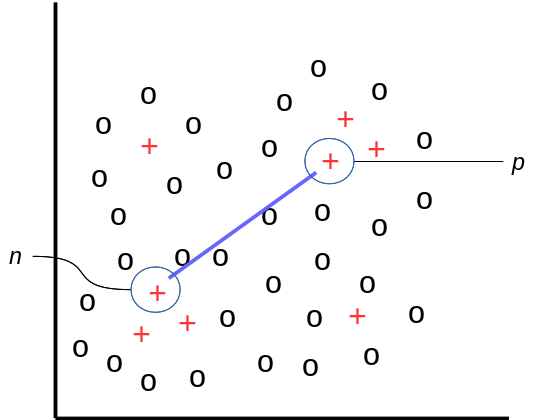
\includegraphics[keepaspectratio=true,scale=0.35]{SMOTE-example}
}
	\caption{
	Ilustrasi pembuatan sampel sintetis pada SMOTE.
	Misalkan $p$ adalah sampel minoritas dan $n$ adalah salah satu dari $k$
	tetangga terdekat dari $p$, maka
	sampel sintetis yang baru akan berada di garis antara $p$ dan $n$.
	}
	\label{fig:smote}
\end{figure}

Sampel sintetis dibuat dengan cara berikut, misalkan $p$ adalah salah satu
sampel minoritas pada dataset $D$,
\pagebreak
\begin{itemize}
	\item Cari $k$ sampel tetangga dari $p$ pada $D$
	\item Untuk setiap sampel tetangga $k$,
	\begin{itemize}
		\item Hitung selisih antara vektor fitur $p$ dengan tetangga $k_{i}$
		\item Kalikan selisih tersebut dengan angka ril acak antara 0 sampai 1,
		dan
		\item simpan hasilnya ke vektor fitur sintentis yang baru.
	\end{itemize}
\end{itemize}

Cara ini membuat sampel secara acak pada segmen garis antara dua fitur yang
terpilih, seperti yang terlihat pada gambar \ref{fig:smote}.
Pendekatan ini secara efektif mendorong wilayah pembelajaran dari kelas
minoritas menjadi lebih besar tanpa menyebabkan \textit{overfitting}.


	\section{LNSMOTE}
	\label{bab:02:lnsmote}
	Meskipun hasil SMOTE dibuktikan bagus dalam makalah Chawla dkk.
\cite{chawla2002smote}, metode ini masih memiliki beberapa kelemahan.
Pertama, cara menentukan sampel minoritas sebagai calon untuk
\textit{over-sampling} bisa bermasalah.
Pada SMOTE, semua sampel dari kelas minoritas digunakan.
Namun, bukan berarti semua sampel tersebut sama bergunanya bagi pembelajaran
klasifikasi.
Pada khususnya, sampel yang ada pada batas \textit{decision}, atau berada
dibatas kelas minoritas dengan kelas mayoritas, lebih sering salah
diklasifikasi dibandingkan dengan sampel yang berada jauh dari batas kelas,
oleh karena itu mereka lebih penting untuk klasifikasi.
Sampel yang jauh dari batas kelas, berada di tengah kelas minoritas mungkin
berkontribusi sedikit pada klasifikasi.
Salah satu metode untuk menangani permasalahan ini yaitu dengan hanya
mengambil sampel pada batas kelas minoritas yang dijadikan untuk
\textit{oversampling}, seperti yang diajukan oleh Han dkk.
\cite{han2005borderline} dengan menggunakan metode bernama \textit{Borderline
SMOTE}.

\begin{figure}[htbp]
	\centering
	\begin{subfigure}[b]{0.4\textwidth}
		\centering
		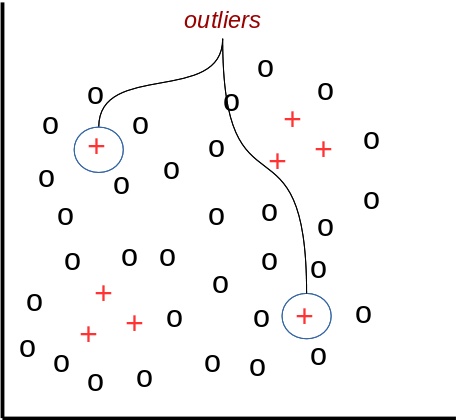
\includegraphics[width=\textwidth]{SMOTE-problem-outliers}
		\caption{}
		\label{fig:smote-outliers}
	\end{subfigure}
	\begin{subfigure}[b]{0.5\textwidth}
		\centering
		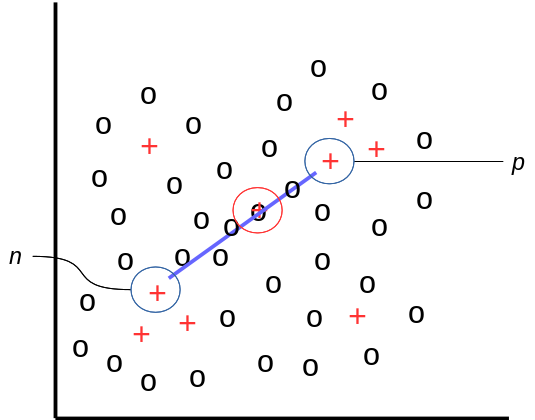
\includegraphics[width=\textwidth]{SMOTE-problem-overlapping}
		\caption{}
		\label{fig:smote-overlapping}
	\end{subfigure}
	\caption{
Kelemahan metode SMOTE:
(a) \textit{Outliers} pada kelas minoritas tidak diperhitungkan pada metode
SMOTE.
(b) Pembuatan sampel sintetis yang baru berada di wilayah kelas mayoritas
yang tumpang-tindih dengan sampel kelas mayoritas.
	}
	\label{fig:smote-problems}
\end{figure}

Kelemahan lain dari SMOTE yaitu permasalahan \textit{overgeneralization} yang
begitu saja menggeneralisasi wilayah dari kelas minoritas.
SMOTE tidak mempertimbangkan distribusi dari sampel pada kelas mayoritas, atau
adanya \textit{outliers}.

Untuk mengatasi permasalahan di atas, Maciejewski dkk. memperkenalkan ekstensi
dari metode SMOTE bernama \textit{Local-neighbourhood SMOTE} atau disingkat
LNSMOTE \cite{maciejewski2011local} yang menggunakan modifikasi dari
pendekatan \textit{Safe-Level SMOTE} \cite{bunkhumpornpat2009safe}.
Pada metode \textit{Safe-level SMOTE} keberadaan sampel mayoritas
diperhitungkan sebelum membuat sampel sintetis dengan menghitung sebuah
koefisien khusus yang disebut \textit{safe level}.
Untuk setiap sampel dari kelas minoritas, dihitung jumlah sampel kelas
minoritas di antara \textit{k-nearest-neighbors} (KNN).
Jika nilainya sama atau mendekati $ 0 $, sampel tersebut dianggap sebagai
\textit{noise}.
Jika nilainya mendekati $ k $, maka sampel tersebut bisa dikatakan berada
di wilayah aman dari kelas minoritas.
Gagasan utamanya adalah membuat sampel sintetis yang dekat dengan wilayah aman.

Lebih rincinya, misalkan $ p $ adalah sampel dari kelas minoritas yang akan
menjadi calon untuk \textit{over-sampling}, maka $ k $ sampel terdekat dengan
$ p $ yang termasuk pada kelas minoritas $ P $ ditentukan.
Seperti pada SMOTE, setidaknya satu dari tetangga tersebut dipilih, sebutlah
dengan $ n $.
Untuk kedua sampel, $ p $ dan $ n $, $ k $ sampel terdekatnya untuk keseluruhan
data pelatihan $ S $ dihitung \textit{safe level}-nya dengan notasi $ sl(p) $
dan $ sl(n) $.
Dari pengetahuan tersebut, koefisien rasio \textit{safe-level} ditentukan
dengan $ \textit{sl-ratio} = sl(p) / sl(n) $.
Langkah selanjutnya ditentukan berdasarkan 5 kasus berikut:
\begin{enumerate}
	\item \label{case:safe-1} Jika $ sl(p) = 0 $ dan $ sl(n) = 0 $, sampel
	$ p $ dan $ n $ dianggap sebagai \textit{noise outliers}, dan tidak ada
	sampel sintetis yang dibuat.
	\item Jika $ sl(p) > 0 $ dan $ sl(n) = 0 $, maka $ n $
	adalah \textit{noise}.
	Sampel sintetis akan dibuat jauh dari $ n $ dengan menduplikasi $ p $.
	\item Jika $ sl-ratio = 1 $, maka $ p $ dan $ n $ memiliki tetangga
	yang sama dan sampel sintetis yang baru akan dibuat diantara garis yang
	menghubungkan mereka dengan cara yang sama seperti pada SMOTE.
	\item Jika $ sl-ratio > 1 $, maka $ p $ berada di wilayah
	aman minoritas daripada $ n $ dan sampel sintetis yang baru akan
	dibuat dekat dengan $ p $, dengan parameter acak pada SMOTE akan
	memiliki rentang $ [0, 1 / \textit{sl-ratio}] $.
	\item Jika \textit{sl-ratio < 1}, maka \textit{n} berada di wilayah
	aman minoritas daripada $ p $ dan sampel sintetis yang baru akan
	dibuat dekat dengan $ n $, yaitu parameter acak pada SMOTE akan
	memiliki rentang $ [1 - \textit{sl-ratio}, 1] $.
\end{enumerate}

Strategi \textit{safe-level SMOTE} bermasalah khususnya pada distribusi kelas
yang bias yang mana kelas minoritas menyebar sehingga terdiri dari beberapa
sub-wilayah dengan kardinalitas yang kecil.
Situasi ini mengacu pada permasalahan yang disebut \textit{small disjuncts}
yang diakui sebagai sumber kesulitan yang paling penting bagi pembelajaran
klasifikasi untuk data timpang \cite{jo2004class}.
Pada kasus seperti ini pembuatan sampel sintetis dengan \textit{Safe-level
SMOTE} bisa menyebabkan terjadinya tumpang-tindih antara kelas.

Sebagai contohnya, misalkan dua kelompok dari kelas minoritas terpisah
dikelilingi oleh sampel dari kelas mayoritas.
Katakanlah, jarak antara kedua kelompok minoritas tersebut cukup jauh, satu
kelompok berada di bawah dan kelompok lainnya di atas.
Misalkan calon dari sebuah sampel berada di kelompok yang dibawah.
Jika parameter $ k $ dari fungsi pencarian KNN lebih besar dari jumlah sampel
kelas minoritas di dalam kelompok tersebut, maka tetangga dari kelas minoritas
selanjutnya akan menjadi sampel dari kelompok yang lain.
Jika rasio \textit{safe-level} dari sampel kedua kelompok sama, sampel sintetis
yang baru bisa dibuat diantara garis yang menggabungkan sampel-sampel dari
kedua kelompok tersebut.
Dengan kata lain, sampel sintetis yang baru bisa berada di wilayah yang dihuni
oleh kelas mayoritas.
Makanya, strategi ini masih memungkinkan terjadinya tumpang-tindih antara
kelas.

Situasi tidak diinginkan seperti di atas disebabkan karena teknik SMOTE mencari
KNN yang dimiliki oleh kelas minoritas saja.
Jika calon sampel tidak berada di wilayah yang padat dengan kelas minoritas,
maka beberapa tetangganya bisa saja cukup jauh dan juga sampel dari kelas
mayoritas mengelilingi calon sampel tersebut.

LNSMOTE mengatasi masalah tumpang tindih ini dengan lebih mempertimbangkan
tetangga sekitar
(\textit{local neighbourhood})
dari calon sampel minoritas yang mungkin bisa memberikan perkiraan dari
keberadaan sampel kelas mayoritas.
Jadi, pencarian sampel yang terlalu jauh sebaiknya dihindarkan.

Modifikasi teknik LNSMOTE terhadap \textit{Safe-Level} SMOTE yaitu,
\begin{itemize}
\item jika calon sampel $ p $ diidentifikasi berada di tetangga terdekat $ k
$ dari $ n $, sampel tersebut tidak langsung dihitung dengan $ sl(n) $ tapi
dicari tetangga dari $ k + 1 $ selanjutnya.
\item Membatasi rentang interval di mana sampel baru secara acak ditempatkan.
Jadi, pada beberapa kasus dari \textit{safe-level}, LNSMOTE tidak menentukan
batas kanan dari interval dengan 1 tapi sebagai ambang batas $\tau < 1$.
Ambang batas tersebut tidak baku tapi ditentukan secara dinamis bergantung
kepada \textit{safe-level} dari sampel mayoritas.
\item Jika $ sl(n) $ relatif rendah, artinya $ n $ dikelilingi oleh banyak
sampel dari kelas mayoritas, sampel baru seharusnya ditempatkan lebih dekat ke
$ p $.
\item Jika $ n $ dikelilingi oleh sejumlah sampel minoritas yang seimbang,
sehingga nilai $ sl(n) $ tinggi, sampel yang baru bisa berada di dekat $ n $.
Hal ini supaya bisa mengontrol tingkat ekspansi dari kelas minoritas dengan
cara dinamis, memperhitungkan distribusi lokal dari sampel.
\end{itemize}

Algoritma LNSMOTE yang digunakan pada implementasi tesis berdasarkan pada
makalah Maciejewski dkk.
\cite{maciejewski2011local}
yang dapat dilihat pada lampiran
\ref{lampiran:alg_lnsmote}.


	\section{\textit{Random Forest}}
	\label{bab:02:rf}
	\textit{Random Forest} (RF) \cite{breiman2001random}
adalah sebuah kombinasi dari beberapa pohon keputusan yang mana setiap pohon
bergantung kepada nilai dari vektor acak yang disampel secara independen dan
dengan distribusi yang sama.

Pohon keputusan yang digunakan dalam RF dapat menggunakan ID3
(\textit{Iterative Dichotomiser}), C4.5 (pengganti dari ID3), atau CART
(\textit{Classification and Regression Trees}).
Dalam tesis ini, dan umumnya pada implementasi RF, menggunakan CART sebagai
pohon keputusan.

Ada tiga parameter utama dalam pembentukan RF.
Parameter pertama yaitu jumlah pohon yang akan dibangun dalam \textit{forest}
(katakanlah $n$),
parameter kedua yaitu persentase dari sampel pelatihan yang digunakan untuk
membangun pohon (katakanlah $b$),
dan parameter ketiga yaitu jumlah fitur acak yang juga digunakan untuk
membangun pohon (katakanlah $m$).
Ketiga parameter diatur sebelum memulai pembangunan RF dan nilainya sama untuk
semua pohon.

Persentase dari sampel pelatihan yang diambil secara acak umumnya dua per tiga
dari sampel keseluruhan, sehingga meninggalkan sepertiganya sebagai
\textit{out-of-bag} (OOB).
Untuk nilai acak fitur $m$, nilai yang biasa digunakan yaitu akar dari jumlah
fitur atau $log$ dari jumlah fitur \cite{breiman2001random}.

Proses pembangunan RF sebagai berikut.
Diasumsikan diberikan sebuah dataset latihan $S$.
Setelah parameter ditentukan, pada saat pembuatan pohon, ambil sampel dari $S$
secara acak tanpa diganti (sampel yang telah diambil bisa terpilih kembali pada
pengambilan acak berikutnya) sejumlah $b$.
Proses ini dikenal juga dengan \textit{bootstraping}.
Sampel yang tidak terpilih disebut dengan \textit{out-of-bag} (OOB), yang
bisa digunakan untuk penghitungan laju galat mis-klasifikasi.
Dari sampel yang terpilih tersebut ambil $m$ buah fitur secara acak, kemudian
bangun pohon dari $m$ fitur dan $b$ sampel acak tersebut tanpa dibersihkan
(\textit{pruning}).
Ulangi proses tersebut sampai pohon ke-$n$.

Proses klasifikasi pada RF berjalan seperti berikut.
Diberikan dataset $T$ yaitu dataset yang berisi fitur yang sama dengan dataset
pelatihan $S$.
Untuk setiap sampel yang akan diklasifikasi pada dataset $T$, masukan sampel
tersebut ke setiap pohon.
Kumpulkan hasil klasifikasi dari setiap pohon, kemudian ambil mayoritas kelas
dari semua hasil klasifikasi tersebut.
Fungsi selengkapnya dari pembuatan dan klasifikasi RF dapat dilihat pada
algoritma \ref{alg:rf}.

\begin{center}
\captionof{algorithm}{Random Forest}
\label{alg:rf}
	\begin{algorithmic}[1]
\Require \\
$ TSET $: dataset pelatihan \\
$ T $: jumlah pohon untuk \textit{forest} \\
$ B $: persentase sampel yang dipilih secara acak tanpa diganti dari $TSET$ \\
$ m $: jumlah fitur acak \\

\Function{RandomForest}{$ TSET, T, B, m $}
	\State $ n \gets $ jumlah sampel pada dataset $ TSET $
	\State $ b \gets n * (B / 100) $
	\Comment Jumlah sampel untuk setiap pohon.

	\State $ forest \gets nil $
	\For{$ t \gets 1,T $}
		\State $ tp, tn, tree \gets \Call{GrowTree}{forest, TSET, b, m} $
		\State $ \Call{forest.Add}{tree} $
	\EndFor
	
	\State \Return $forest$
\EndFunction
\\
\Function{GrowTree}{$ forest, TSET, b, m $}
	\label{bagging}
	\State $ bag, oob, bagIdx, oobIdx \gets \Call{RandomPickSample}{$ TSET,
	b $} $

	\State $ tree \gets \Call{BuildTree}{bag, m} $

	\State $ \Call{forest.SaveBagIndex}{bagIdx} $
	\Comment Simpan pohon dan indeks dari \textit{bagging}

	\State $ cm \gets \Call{Classify}{forest, oob, oobIdx} $
	\State $ tp, tn \gets \Call{ComputeStat}{cm} $
	\Comment Hitung laju galat OOB dari \textit{confusion matrix}
	$cm$.

	\State \Return{$ tp, tn, tree $}
\EndFunction
\\
\Function{Classify}{$ forest, set, setIdx $}
	\State $ predictions \gets nil $
	\For{\textbf{each} $ sample, idx $ \textbf{in} $ set $}
		\State $ votes \gets \Call{ForestVotes}{forest, sample, idx} $
		\State $ class \gets \Call{Majority}{votes} $
		\Comment ambil mayoritas suara kelas pada $votes$
		\State $ predictions.push(class) $
	\EndFor

	\State \Return $predictions$
\EndFunction
\\
\Function{ForestVotes}{$ forest, sample, idx $}
	\State $ votes \gets nil $
	\For{\textbf{each} $ tree $ \textbf{in} $forest$ }
		\State $ exist \gets \Call{IsSampleInTheBag}{idx} $
		\Comment Periksa apakah sampel indeks digunakan pada pohon ini.

		\If{exist}
			\State continue
			\Comment Jika digunakan, lanjutkan ke pohon berikutnya.
		\EndIf

		\State $ class \gets \Call{tree.Classify}{sample} $

		\State $ \Call{votes.push}{class} $
	\EndFor

	\State \Return $ votes $
\EndFunction
	\end{algorithmic}
\end{center}



	\section{\textit{Cascaded Random Forest}}
	\label{bab:02:crf}
	Permasalahan umum dalam penggalian data atau algoritma pembelajaran ansambel
adalah ketidakmampuan untuk menangani data pelatihan yang timpang.
Ketimpangan antara kelas positif dan negatif biasanya menyebabkan akurasi
deteksi yang rendah.
Simulasi yang dilakukan oleh Strobel dkk. \cite{strobl2007bias} menampilkan
bahwa RF condong mendukung kelas mayoritas.
Saat menggunakan RF untuk deteksi, sejumlah besar sampel negatif dibutuhkan
untuk mendapatkan pengklasifikasi yang kuat dan laju \textit{false-positive}
yang rendah.
Hal ini menyebabkan ketimpangan yang besar antara kelas positif dan
negatif, sehingga membuat pengklasifikasi RF yang berfokus pada kelas
mayoritas.
Kelemahan lain dari RF yaitu setelah belajar dengan beberapa pohon, RF secara
gradual mencapai titik puncaknya, yang mana pengklasifikasi tidak bisa lagi
meningkatkan \textit{sensitivity} pada pendeteksian maupun mengurangi laju
\textit{false-positive}-nya.

Pada tahun 2011, Viola dan Jones mengajukan algoritma deteksi sampel cepat
berbasis AdaBoost dengan struktur kaskade (\textit{cascade})
\cite{viola2004robust}.
Struktur kaskade dimotivasi oleh asumsi bahwa lebih mudah untuk menolak sebuah
sampel yang negatif daripada mencari sampel yang positif.
Viola dan Jones menggabungkan pengklasifikasi yang kuat pada beberapa tingkatan
yang independen dengan kondisi bahwa setiap tingkat dapat menolak sebuah
sampel, sehingga supaya sebuah sampel dapat dianggap positif semua tingkat
harus terlewati.
Disebabkan karena dominasi penolakan pada tahap-tahap awal, waktu komputasi
menjadi berkurang.
Sebagai tambahan, untuk mendapatkan pelatihan yang lebih baik, Viola dan Jones
mengajukan strategi \textit{bootstrap} dengan menghapus sampel yang benar
terklasifikasi negatif setelah pembelajaran dilakukan pada setiap tingkat.
Setelah itu, dataset pelatihan yang berkurang ditambahkan dengan sampel yang
salah diklasifikasi (\textit{false-positive})
\cite{viola2004robust}.

Sebuah pengklasifikasi kaskade terdiri dari sejumlah tingkatan dengan
kompleksitas yang meningkat.
Setiap tingkat minimum memiliki satu pengklasifikasi independen.
Pengklasifikasi ditambahkan ke dalam tingkatan sampai batas nilai
\textit{true-positive} dan \textit{true-negative} tercapai.
Keuntungan dari struktur kaskade yaitu sejumlah besar sampel dapat
didistribusikan diantara tingkatan, berkurangnya nilai \textit{false-positive},
dan berkurangnya waktu komputasi baik pada pelatihan dan klasifikasi.

Baumann menerapkan metoda ini pada RF dan mengajukan \textit{Cascaded Random
Forest} (CRF) yaitu penggabungan dari pengklasifikasi RF dengan struktur
kaskade, yang menyusun beberapa pohon keputusan dalam setiap tingkatan dengan
strategi agregasi \textit{bootstrap}.
Sehingga, pembelajaran pada sampel positif meningkat dan kelemahan dari data
yang timpang terhindari \cite{baumann2013cascaded}.

Pengklasifikasi CRF memiliki enam parameter umum, tiga diantaranya sama dengan
RF yaitu jumlah pohon ($T$), persentase sampel acak untuk \textit{bootstrap},
($b$), dan jumlah fitur acak ($m$).
Tiga parameter lainnya yaitu jumlah tingkatan ($S$), nilai ambang batas
\textit{true-positive} ($maxtp$), dan nilai ambang batas
\textit{true-negative} ($maxtn$).

Strategi \textit{bootstrap} yang digunakan adalah sebagai berikut: setelah
menyelesaikan pembelajaran pada sebuah tingkatan, dataset pelatihan yang berisi
hanya sampel negatif diujikan ke semua tingkatan yang telah dibentuk
sebelumnya dengan tujuan untuk menghapus sampel yang benar bernilai
\textit{true-negative} saja, sehingga dataset pelatihan sebisa mungkin berisi
hanya sampel positif.
Sampel yang terklasifikasi \textit{false-positive} kemudian dimasukan kembali
ke dataset pelatihan untuk dipelajari oleh tingkatan berikutnya.
Fungsi selengkapnya dari CRF dapat dilihat pada algoritma \ref{alg:crf}.

Beberapa tingkatan memiliki akurasi deteksi yang lebih rendah daripada
yang lainnya.
Untuk mengurangi pengaruh tingkatan yang memiliki performansi yang rendah
tersebut, maka dihitung faktor bobot $\alpha$ dari setiap tingkatan dengan
mengeksploitasi rerata harmonik dari \textit{precision} dan \textit{recall},
atau dikenal juga dengan nilai $F_1$ (\textit{fmeasure}),
pada dataset pelatihan.

Nilai $\alpha$ pada setiap tingkatan secara linear dinormalisasi pada rentang 0
dan 1, sehingga bobot dari tingkat yang memiliki performansi yang rendah
berkurang supaya pengaruhnya terhadap mayoritas \textit{voting} juga berkurang.
Proses untuk mendapatkan hasil dari pengklasifikasi CRF diberikan pada gambar
\ref{form:crf}.

\begin{figure}[h]
\[
	y(x) = argmax \left(
			\frac{1}{T \cdot \sum^{S}_{s=1} \alpha_{s} }
			\sum\limits_{s=1}^{S} \alpha_{s}
			\sum\limits^{T}_{t=1} I_{h_{t} (x) = c}
		\right)
\]
\caption{
Formula untuk mendapatkan kelas (\textit{voting}) pada pengklasifikasi CRF
dengan bobot.
}
\label{form:crf}
\end{figure}

Pada gambar \ref{form:crf}, $x$ adalah sampel yang akan diklasifikasi,
$S$ adalah jumlah tingkatan pada struktur kaskade,
$\alpha_{s}$ adalah nilai bobot dari tingkatan,
$T$ adalah jumlah pohon pada tingkatan, dan
$h_{t}$ yaitu fungsi klasifikasi dari sebuah pohon yang memberikan sebuah nilai
kelas $c$ yang bisa memiliki nilai indikator dari $I$
(misalkan nilai 1 untuk positif atau 0 untuk negatif).


	\section{Pekerjaan Terkait}\label{bab:02:pekerjaan_terkait}
	Deteksi vandalisme di Wikipedia berbasis pendekatan pembelajaran mesin telah
menjadi topik penelitian yang menarik sejak tahun 2008.
\textcite{potthast2008automatic} berkontribusi untuk pendekatan deteksi
vandalisme dengan pembelajaran mesin yang pertama, dengan menggunakan fitur
tekstual berikut fitur meta data dasar dengan menggunakan pengklasifikasi
\textit{logistic regression}.
\textcite{smets08automaticvandalism} menggunakan pengklasifikasi Naive Bayes
pada sekumpulan kata yang merepresentasikan suntingan dan yang pertama
menggunakan model kompresi untuk mendeteksi vandalisme di Wikipedia.
\textcite{itakura2009using} menggunakan Kompresi Markov Dinamis
untuk mendeteksi suntingan vandalisme di Wikipedia.
\textcite{mola2012wikipedia} mengembangkan pendekatan yang dilakukan
oleh \textcite{potthast2008automatic} dengan menambahkan beberapa fitur
tekstual dan berbagai fitur berbasis daftar-kata.
Velasco memenangi \textit{1st International Competition on Wikipedia Vandalism
Detection}.
\textcite{west2011multilingual} adalah yang pertama
mengajukan pendekatan deteksi hanya berdasarkan meta data
spasial dan temporal, tanpa perlu memeriksa teks pada artikel dan revisi.
\textcite{adler2010detecting} membangun sebuah sistem deteksi vandalisme
menggunakan sistem reputasi WikiTrust.
\textcite{adler2011wikipedia} kemudian menggabungkan bahasa alami,
spasial, temporal, dan fitur reputasi yang digunakan pada karya sebelumnya.
\textcite{west2011multilingual} adalah yang pertama memperkenalkan
data \textit{ex post facto} sebagai fitur, yang mana perhitungannya
mempertimbangkan revisi selanjutnya.
Sistem deteksi vandalisme West dan Lee memenangkan \textit{2nd International
Competition on Wikipedia Vandalism Detection}.
\textcite{harpalani2011language} menyatakan suntingan vandalisme
memiliki properti lingustik yang unik dan sama.
Harpalani dkk. membangun sistem deteksi vandalisme berdasarkan analisis
\textit{stylometric} dari suntingan vandalisme dengan model probabilitas
\textit{context-free grammar}.
Pendekatan Harpalani dkk. mengalahkan sistem berbasis fitur dengan pola
dangkal, yang menyamakan struktur sintaksis dan token teks.
Mengikuti tren dari klasifikasi vandalisme antar bahasa,
\textcite{tran2013cross} mengevaluasi berbagai pengklasifikasi berbasiskan pada
sekumpulan fitur independen bahasa yang dikumpulkan dari jumlah artikel dilihat
setiap jam dan riwayat suntingan Wikipedia.

\textcite{gotze2014advanced} menggabungkan fitur dari
\textcite{adler2011wikipedia},
\textcite{javanmardi2011vandalism},
\textcite{mola2012wikipedia},
\textcite{potthast2008automatic},
\textcite{wang2010got}, dan
\textcite{west2011multilingual} dengan empat fitur tambahan dan perubahan.
Untuk mengatasi masalah ketimpangan pada korpus,
\textcite{gotze2014advanced}
mengaplikasikan teknik
\textit{random oversampling}
bernama
\textit{Synthetic Minority Over-sampling TEchnique} (SMOTE)
yang diajukan oleh
\textcite{chawla2002smote},
dan kombinasi dari SMOTE dan
\textit{random undersampling}.
Dataset latihan yang orisinal dan hasil sampel ulang diuji dengan
pengklasifikasi satu-kelas dan dua-kelas.
Pengklasifikasi satu-kelas yang diterapkan diantaranya
\textcite{hempstalk2008one}
dan SVM oleh
\textcite{scholkopf1999support}
yang diimplementasikan oleh
\textcite{chang2011libsvm}
pada korpus PAN-WVC.
Pengklasifikasi dua-kelas yang diterapkan diantaranya
\textit{Logistic Regression},
\textit{RealAdaBoost},
\textit{Random Forest} (RF), dan
\textit{Bayesian Network}.
Hasil percobaan yang didapat memperlihatkan performansi pengklasifikasi
satu-kelas tidak kompetitif dengan satu pun pengklasifikasi dua-kelas.
Hal ini bisa disebabkan karena tidak sesuainya kelompok fitur yang digunakan
untuk menjelaskan suntingan vandalisme, sebagaimana juga parameter pengaturan
yang tidak sesuai pada pendekatan yang digunakan.
Hasil dari pelatihan pada dataset orisinal memperlihatkan RF
lebih unggul dari pengklasifikasi lainnya.
Hasil dari pelatihan pada dataset hasil sampel ulang memperlihatkan adanya
peningkatan pada semua pengklasifikasi kecuali pada RF.



Dari penelitian di atas, tujuh diantaranya menggunakan PAN-WVC-10
\parencites{adler2010detecting}
{adler2011wikipedia}
{gotze2014advanced}
{harpalani2011language}
{mola2012wikipedia}
{wang2010got}
{west2011multilingual},
dengan nilai presisi terbaik yaitu $0,86$, nilai \textit{recall} $0,57$, dan
PR-AUC $0,66$ didapat oleh Velasco menggunakan \textit{Random Forest} tanpa
penyeimbangan dataset.
Hanya dua yang menggunakan PAN-WVC-11
\parencites{gotze2014advanced}
{west2011multilingual}
dengan hasil terbaik dipegang oleh Gotze yaitu
dengan nilai presisi $0,92$, \textit{recall} $0,39$, dan PR-AUC $0,74$.


	\section{Fitur Vandalisme}
	\label{bab:02:fitur_vandalisme}
	Beberapa makalah sebelumnya mengelompokan fitur ke dalam tiga kelompok yaitu
\textit{metadata}, teks, dan bahasa.
Dalam tesis ini digunakan 4 fitur metadata, 11 fitur teks, dan 10 fitur
bahasa yang diambil dari hasil analisis makalah
\textcite{mola2012wikipedia}.

\subsubsection{Fitur Kelompok Metadata}

Kelompok metadata mengacu pada properti dari sebuah revisi yang secara langsung
dapat diambil, seperti identitas penyunting, komentar, atau ukuran perubahan.

Berikut daftar fitur metadata yang digunakan,

\begin{itemize}

\item \textbf{Anonim}.
Penyunting anonim yaitu yang tidak menggunakan akun Wikipedia saat melakukan
penyuntingan, sehingga yang tercatat hanya alamat IP bukan nama pengguna.
Fitur ini melihat apakah suntingan anonim atau bukan pada atribut
\textit{editor}, jika benar maka ditandai dengan nilai 1, atau 0 sebaliknya.
Vandal lebih condong berlaku anonim karena jika menggunakan akun asli akan
membuat akun mereka mudah diblokir dan membuat akun baru membutuhkan waktu dan
identitas berupa alamat surel.

\item \textbf{Panjang komentar}.
Melihat dari jumlah karakter yang diinputkan di kolom rangkuman suntingan, yang
tersimpan dalam atribut \textit{editcomment} pada dataset, saat menyimpan hasil
suntingan, tanpa mengikutkan bagian \textit{header} yaitu penanda di awal
komentar yang menunjuk ke bagian yang di sunting, biasanya dalam format
"\texttt{/* Nama header */}".
Komentar yang panjang mungkin mengindikasikan suntingan normal dan yang pendek
atau kosong mungkin menyarankan suatu vandalisme.

\pagebreak

\item \textbf{Peningkatan ukuran}.
Peningkatan absolut dari ukuran konten artikel.
Berkurangnya ukuran dalam jumlah besar bisa mengindikasikan
pengosongan artikel. Fitur ini dihitung dengan,
\begin{equation}
|\text{Ukuran suntingan baru} - \text{Ukuran suntingan lama}|
\end{equation}

\item \textbf{Rasio ukuran}.
Ukuran revisi baru relatif terhadap revisi lama.
Pada suntingan biasa, penghapusan biasanya diikuti dengan sejumlah perbaikan.
Fitur ini mendeteksi dengan menghitung penambahan atau penghapusan yang
berlebihan, dengan cara

\begin{equation}
\frac{1 + |\text{Ukuran suntingan baru}|}{1 + |\text{Ukuran suntingan lama}|}
\end{equation}

\end{itemize}


\subsubsection{Fitur Kelompok Teks}

Berikut daftar fitur berbasiskan teks yang digunakan,

\begin{itemize}

\item \textbf{Rasio huruf besar dan kecil}.
Pelaku vandal biasanya tidak mengikuti aturan huruf kapital, menulis semuanya
dengan huruf kecil atau huruf besar.
Rasio ini dihitung pada teks yang ditambahkan di revisi baru dengan menggunakan
rumus

\begin{equation}
\frac{1 + |\text{Jumlah huruf besar}|}{1 + |\text{Jumlah huruf kecil}|}
\end{equation}

\item \textbf{Rasio huruf besar terhadap semua karakter}
Rasio ini dihitung dengan menggunakan rumus

\begin{equation}
\frac{1 + |\text{Jumlah huruf besar}|}%
	{1 + |\text{Jumlah huruf besar}| + |\text{Jumlah huruf kecil}|}
\end{equation}

\item \textbf{Rasio angka}.
Rasio semua karakter terhadap angka, yaitu

\begin{equation}
\frac{1 + |\text{Jumlah karakter angka}|}{1 + |\text{Jumlah semua karakter}|}
\end{equation}

Fitur ini membantu menemukan perubahan kecil yang hanya mengubah angka.
Contoh kasusnya perubahan sebuah tanggal atau perhitungan yang disengaja untuk
memberikan informasi yang salah.

\item \textbf{Rasio non-alfanumerik}.
Rasio semua karakter terhadap karakter selain huruf dan angka, yaitu

\begin{equation}
\frac{1 + |\text{Jumlah karakter non alfanumerik}|}%
	{1 + |\text{Jumlah semua karakter}|}
\end{equation}

Penggunaan karakter selain angka-huruf yang berlebihan bisa mengindikasikan
penggunaan \textit{emoticon}, tanda baca, atau kata tak bermakna.

\item \textbf{Diversitas karakter}.
Menghitung jumlah karakter berbeda yang digunakan pada penambahan, dibandingkan dengan panjang teks yang dimasukan,
dihitung dengan rumus,

\begin{equation}
\text{panjang teks}^{\frac{1}{1+\text{karakter unik}}}
\end{equation}

Fitur ini membantu menemukan penggunaan karakter secara acak dan kata tak
bermakna.

\item \textbf{Distribusi karakter}.
Menggunakan Divergensi Kullback-Leibler dari distribusi karakter yang dimasukan
terhadap ekspektasi.
Fitur ini berguna untuk mendeteksi kata tak bermakna.

\item \textbf{Laju kompresi}.
Melihat tingkat kompresi dari penambahan teks menggunakan algoritma kompresi
LZW.
Fitur ini berguna untuk mendeteksi kata tak bermakna, pengulangan kata atau
karakter, dll.
Vandalisme biasanya memiliki ukuran kompresi yang rendah.

\item \textbf{Token umum}.
Menghitung token yang biasanya jarang digunakan oleh vandal yaitu sintaks
wiki, seperti \textit{\_\_TOC\_\_}. Daftar token dapat dilihat pada lampiran
\ref{lampiran:words_wiki_token}.

\item \textbf{Frekuensi rerata kata}.
Frekuensi relatif rerata dari kata yang dimasukan pada revisi baru.
Pada artikel yang panjang, semakin banyak kata yang dimasukan yang tidak ada
pada artikel mengindikasikan bahwa suntingan tersebut bisa tak bermakna atau
tidak berhubungan dengan isinya.

\item \textbf{Kata terpanjang}.
Panjang dari kata yang dimasukan.
Nilainya akan 0 jika tidak ada kata yang dimasukan.
Fitur ini berguna untuk mendeteksi suntingan tak-bermakna.

\item \textbf{Urutan karakter terpanjang}.
Urutan terpanjang dari karakter yang sama pada teks yang dimasukan sering
digunakan pada vandalisme, contohnya \textit{aaarrrrggghhh! sooo huge}.

\end{itemize}

\subsubsection{Fitur Kelompok Bahasa}

Fitur kelompok bahasa didasarkan pada jumlah kata tertentu yang ditambahkan
pada suntingan atau revisi yang baru.
Untuk setiap kategori kata dihitung dua jenis fiturnya: frekuensi dan impak.

Fitur frekuensi yaitu menghitung frekuensi dari kategori kata terhadap
total seluruh kata pada suntingan yang baru, yaitu

\begin{equation}
	\frac{\text{Jumlah kategori kata}}
		{\text{Jumlah seluruh kata}}
\end{equation}

Fitur impak yaitu menghitung persentase peningkatan kategori kata di revisi
yang baru, dihitung dengan,

\begin{equation}
	\frac{\text{Jumlah kata di revisi lama}}%
		{
			\text{Jumlah kata di revisi lama} +
			\text{Jumlah kata di revisi baru}
		}
\end{equation}

Berikut daftar kategori kata yang digunakan,

\begin{itemize}
\item \textbf{Vulgarisme}.
Menghitung kata-kata vulgar, kasar dan menghina.
Daftar kategori kata ini dapat dilihat pada lampiran
\ref{lampiran:words_vulgar}.

\item \textbf{Subjek}.
Menghitung kata subjek pertama atau kedua, termasuk pengejaan tidak baku,
misalnya \textit{I}, \textit{you}, \textit{ya}.
Daftar kategori kata ini dapat dilihat pada lampiran
\ref{lampiran:words_pronoun}.

\item \textbf{Bias}.
Menghitung penggunaan kata sehari-hari yang mengandung bias, misalnya
\textit{coolest}, \textit{huge}.
Daftar kategori kata ini dapat dilihat pada lampiran
\ref{lampiran:words_bias}.

\item \textbf{Pornografi}.
Menghitung penggunaan kata berhubungan dengan pornografi.
Daftar kategori kata ini dapat dilihat pada lampiran
\ref{lampiran:words_sex}.

\item \textbf{Kata buruk}.
Menghitung penggunaan kata sehari-hari dan beberapa penulisan yang buruk
(misalnya, \textit{wanna}, \textit{gotcha}).
Daftar kategori kata ini dapat dilihat pada lampiran
\ref{lampiran:words_bad}.

\item \textbf{Seluruh kategori kata}.
Gabungan dari kategori kata vulgarisme, subjek, bias, pornografi, dan kata
buruk.

\end{itemize}




%%
%% BAB III: PROSES
%%
Pada bab ini dijelaskan proses dari pengolahan dataset dan implementasi
algoritma sampel ulang dan klasifikasi, dimulai dari persiapan
data, pembuatan dataset fitur, sampel ulang pada dataset fitur, dan
implementasi pengklasifikasi sehingga nantinya dapat digunakan untuk pelatihan,
pengujian dan analisis.
Alur dari proses secara umum dapat dilihat pada gambar \ref{fig:proses}.


%%
%% BAB IV: EVALUASI
%%
\chapter{Evaluasi}
\label{bab:04}
Dalam deteksi vandalisme, menemukan sebuah suntingan yang vandal dengan tingkat
positif yang tinggi lebih baik daripada salah klasifikasi atau terlewatnya
suntingan vandal tersebut dari pendeteksian.
Kesalahan klasifikasi, yang bukan vandalisme terdeteksi sebagai vandalisme,
tidak akan berpengaruh pada pembaca, tetapi terlewatnya suntingan yang vandal
bisa menyebabkan hilangnya informasi, kesalahan informasi, atau mengganggu
pembaca Wikipedia.
Oleh karena itu, hasil pelatihan dan pengujian dilihat dari laju
\textit{true-positive} pada performansi.
Laju \textit{true-positive}, atau dikenal juga dengan
\textit{true-positive rate} (TPR),
yaitu total jumlah sampel yang benar positif dibagi dengan
jumlah sampel yang terklasifikasi benar positif (\textit{true-positive})
ditambah dengan jumlah sampel positif terklasifikasi dengan negatif
(\textit{false-negative}).
TPR bernilai dengan rentang antara 0 sampai 1, dengan nilai yang mendekati 0
berarti performansi yang buruk dan nilai yang mendekati 1 berarti performansi
yang baik.
Hasil pengujian diberikan dalam bentuk performansi pengklasifikasi pada tabel
\ref{tab:stats} dan kecepatan pelatihan model pada gambar \ref{graph:runtimes}.

\DTLsetseparator{;}
\DTLloaddb{stats}{../result/stats.csv}

\DTLmaxforcolumn{stats}{TPR}{\maxtpr}
\DTLminforcolumn{stats}{FPR}{\minfpr}
\DTLmaxforcolumn{stats}{TNR}{\maxtnr}
\DTLmaxforcolumn{stats}{Presisi}{\maxprec}
\DTLmaxforcolumn{stats}{F-Measure}{\maxfm}
\DTLmaxforcolumn{stats}{Akurasi}{\maxacc}
\DTLmaxforcolumn{stats}{AUC}{\maxauc}

\begin{table}[htbp]
\caption{Performansi Klasifikasi RF dan CRF}
\centering
\footnotesize
\begin{tabular}{l l r}
\hline
\textbf{Klasifikasi} &
\textbf{Dataset} &
\textbf{TPR}
\DTLforeach*{stats}{%
	\cl=Klasifikasi,%
	\ds=Dataset,%
	\tpr=TPR%
}{%
	\DTLifnullorempty{\cl}
		{\\ \cline{2-3}}
		{\\ \hline \hline}
	\DTLifnullorempty{\cl}
		{}
		{
			\multirow{3}{*}{\cl}
		}
	& \ds
	& \DTLifnumeq{\tpr}{\maxtpr}{\textbf{\tpr}}{\tpr}
}
\\
\hline
\end{tabular}
\label{tab:stats}
\end{table}


Pengklasifikasi CRF dengan 200 tingkat 1 pohon pada dataset yang telah disampel
ulang dengan LNSMOTE memberikan nilai TPR paling tinggi yaitu $0,9904$.
Pengklasifikasi RF tanpa sampel ulang memberikan nilai TPR paling rendah yaitu
$0,1654$.

\begin{figure}[htb]
\centering
\mytikzinput{graph_runtimes}
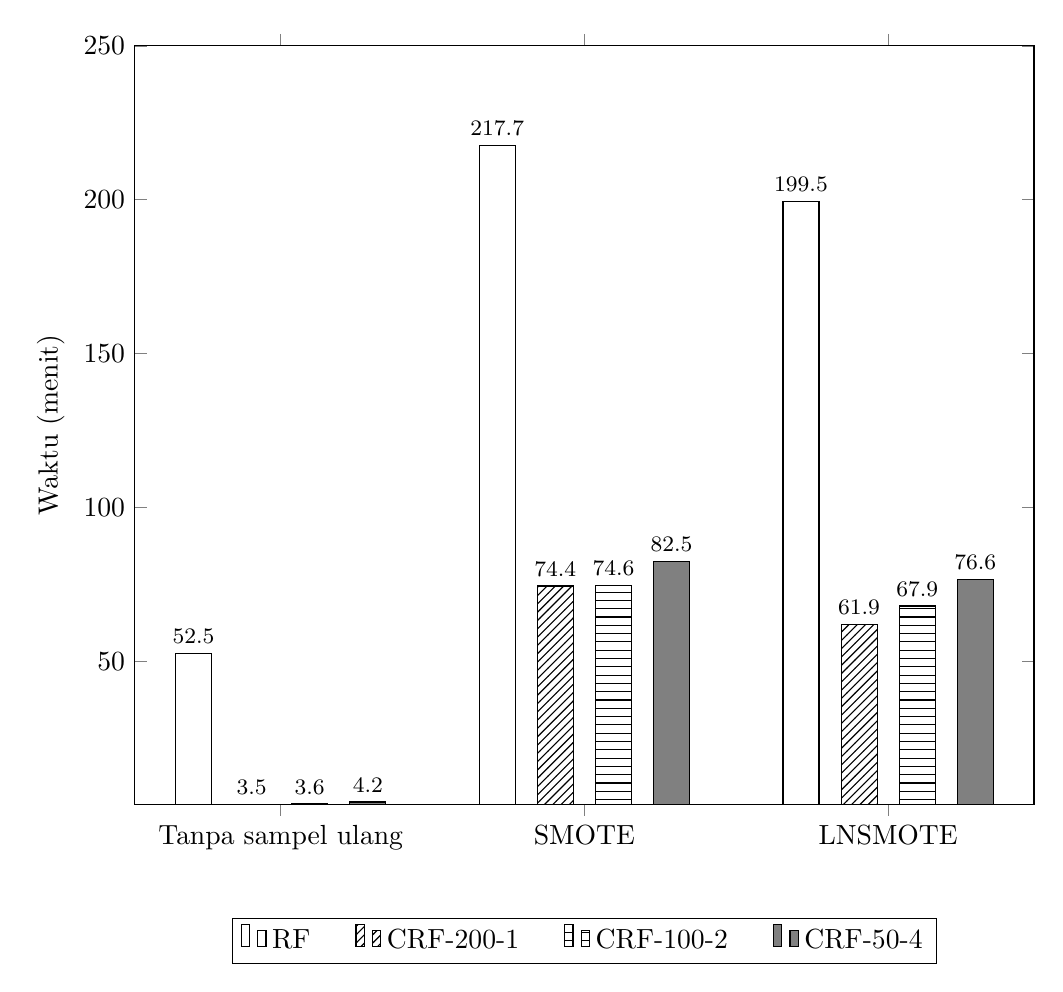
\begin{tikzpicture}
	\begin{axis}[
		width=13cm,
		ymax=250,
		ybar=8pt,
		ylabel=Waktu (menit),
		symbolic x coords={Tanpa sampel ulang, SMOTE, LNSMOTE},
		xtick=data,
		nodes near coords,
		every node near coord/.append style={font=\footnotesize},
		enlarge x limits=0.24,
		enlarge y limits=0,
		bar width = 13pt,
		legend style={
			at={(0.5,-0.15)},
			anchor=north,
			legend columns=-1,
			/tikz/every even column/.append style={column sep=0.5cm}
		},
	]
		%% RF
		\addplot[fill=white] coordinates {
			(Tanpa sampel ulang, 52.5)
			(SMOTE, 217.7)
			(LNSMOTE, 199.5)
		};

		%% CRF-200-1
		\addplot[pattern=north east lines] coordinates {
			(Tanpa sampel ulang, 3.5)
			(SMOTE, 74.4)
			(LNSMOTE, 61.9)
		};

		%% CRF-100-2
		\addplot[pattern=horizontal lines] coordinates {
			(Tanpa sampel ulang, 3.6)
			(SMOTE, 74.6)
			(LNSMOTE, 67.9)
		};

		%% CRF-50-4
		\addplot coordinates {
			(Tanpa sampel ulang, 4.2)
			(SMOTE, 82.5)
			(LNSMOTE, 76.6)
		};
	\legend{RF, CRF-200-1, CRF-100-2, CRF-50-4}
	\end{axis}
\end{tikzpicture}
\caption{Waktu pelatihan untuk setiap klasifikasi berdasarkan dataset.}
\label{graph:runtimes}
\end{figure}


Dari segi kecepatan pelatihan model, pengklasifikasi CRF lebih cepat dari RF
baik pada semua dataset pelatihan.
Sebagai pembanding, dapat dilihat pada klasifikasi RF dan CRF 50 tingkat 4
pohon.
CRF tanpa sampel ulang lebih cepat 11 kali daripada RF, dan pada sampel ulang
SMOTE dan LNSMOTE, klasifikasi CRF 1,6 kali lebih cepat daripada RF.


	\section{Dataset Pelatihan dan Pengujian}
	\label{bab:04:dataset}
	Dataset yang digunakan untuk pelatihan model yaitu PAN-WVC-10 yang terdiri dari
tiga jenis yaitu dataset tanpa sampel ulang, dataset yang telah disampel ulang
dengan SMOTE, dan dataset yang telah disampel ulang dengan LNSMOTE.
Jumlah sampel pada dataset yang tidak disampel yaitu 2.394 positif dan 30.045
negatif dengan total 32.439 sampel.
Jumlah sampel positif pada dataset hasil sampel ulang dengan SMOTE yaitu 28.728
sampel dengan total 58.773 sampel.
Jumlah sampel positif pada dataset hasil sampel ulang dengan LNSMOTE yaitu
28.588 sampel dengan total 58.633 sampel.

\begin{table}[!ht]
\centering
\caption{Dataset untuk pelatihan dan pengujian.}
\begin{tabular}{|| c | l | c | c | c ||}
\hline
\multirow{2}{*}{Tipe} & \multirow{2}{*}{Mode sampel ulang} & \multicolumn{3}{c||}{Jumlah sampel} \\
\cline{3-5}
                         &                                       & Vandalisme & Biasa & Total \\
\hline
\hline
\multirow{3}{*}{Pelatihan} & -       &  2.394 & 30.045 & 32.439 \\
                              & SMOTE   & 27.728 & 30.045 & 58.773 \\
                              & LNSMOTE & 28.588 & 30.045 & 58.633 \\
\hline
Pengujian & - & 1.143 & 8.842 & 9.985 \\
\hline
\end{tabular}
\label{table:dataset}
\end{table}

Dataset yang digunakan untuk pengujian model yaitu PAN-WVC-11 yang terdiri dari
1.143 sampel positif dan 8.842 sampel negatif dengan total 9.985 sampel.
Jumlah fitur pada PAN-WVC-11 sama dengan PAN-WVC-10 yaitu 26 fitur.


	\section{Parameter Pengklasifikasi}
	\label{bab:04:parameter}
	Supaya konsisten antara pengklasifikasi, digunakan parameter umum yang sama
yaitu 200 pohon, 5 (dari $\sqrt{26}$) fitur acak, dan $ 64\% $ untuk
\textit{bootstrapping}.
Untuk klasifikasi CRF dilakukan tiga pemodelan dan pengujian dengan parameter
yang berbeda yaitu 200 tingkat dengan 1 pohon, 100 tingkat dengan 2 pohon, dan
50 tingkat dengan 4 pohon; dengan jumlah pohon yang tetap sama untuk ketiganya
yaitu 200.
Hal ini dilakukan untuk melihat pengaruh dari jumlah pohon terhadap tingkat dan
hasil klasifikasi.
Parameter lain pada pemodelan CRF yaitu nilai ambang batas TPR dan TNR diset
pada nilai $0,95$ dan $0,95$ untuk mendapatkan hasil klasifikasi yang bagus dan
jumlah pohon yang konsisten.


	\section{Hasil Deteksi}
	\label{bab:04:hasil_deteksi}
	\DTLsetseparator{;}
\DTLloaddb{stats}{../result/stats.csv}

\DTLmaxforcolumn{stats}{TPR}{\maxtpr}
\DTLminforcolumn{stats}{FPR}{\minfpr}
\DTLmaxforcolumn{stats}{TNR}{\maxtnr}
\DTLmaxforcolumn{stats}{Presisi}{\maxprec}
\DTLmaxforcolumn{stats}{F-Measure}{\maxfm}
\DTLmaxforcolumn{stats}{Akurasi}{\maxacc}
\DTLmaxforcolumn{stats}{AUC}{\maxauc}

\begin{table}[htbp]
\caption{Performansi Klasifikasi RF dan CRF}
\centering
\footnotesize
\begin{tabular}{l l r}
\hline
\textbf{Klasifikasi} &
\textbf{Dataset} &
\textbf{TPR}
\DTLforeach*{stats}{%
	\cl=Klasifikasi,%
	\ds=Dataset,%
	\tpr=TPR%
}{%
	\DTLifnullorempty{\cl}
		{\\ \cline{2-3}}
		{\\ \hline \hline}
	\DTLifnullorempty{\cl}
		{}
		{
			\multirow{3}{*}{\cl}
		}
	& \ds
	& \DTLifnumeq{\tpr}{\maxtpr}{\textbf{\tpr}}{\tpr}
}
\\
\hline
\end{tabular}
\label{tab:stats}
\end{table}


SMOTE rata-rata meningkatkan nilai TPR $0,19$ kali.
Sementara pada sampel ulang dengan LNSMOTE, rata-rata meningkatkan nilai TPR
$0,33$ kali.
Pengklasifikasi CRF dengan 200 tingkat 1 pohon pada dataset yang telah disampel
ulang dengan LNSMOTE memberikan nilai TPR paling tinggi.
Pengklasifikasi RF tanpa sampel ulang memberikan nilai TPR paling rendah.
Hasil pengujian secara keseluruhan dapat dilihat pada tabel \ref{tab:stats}

\begin{figure}[htb]
\centering
\mytikzinput{graph_runtimes}
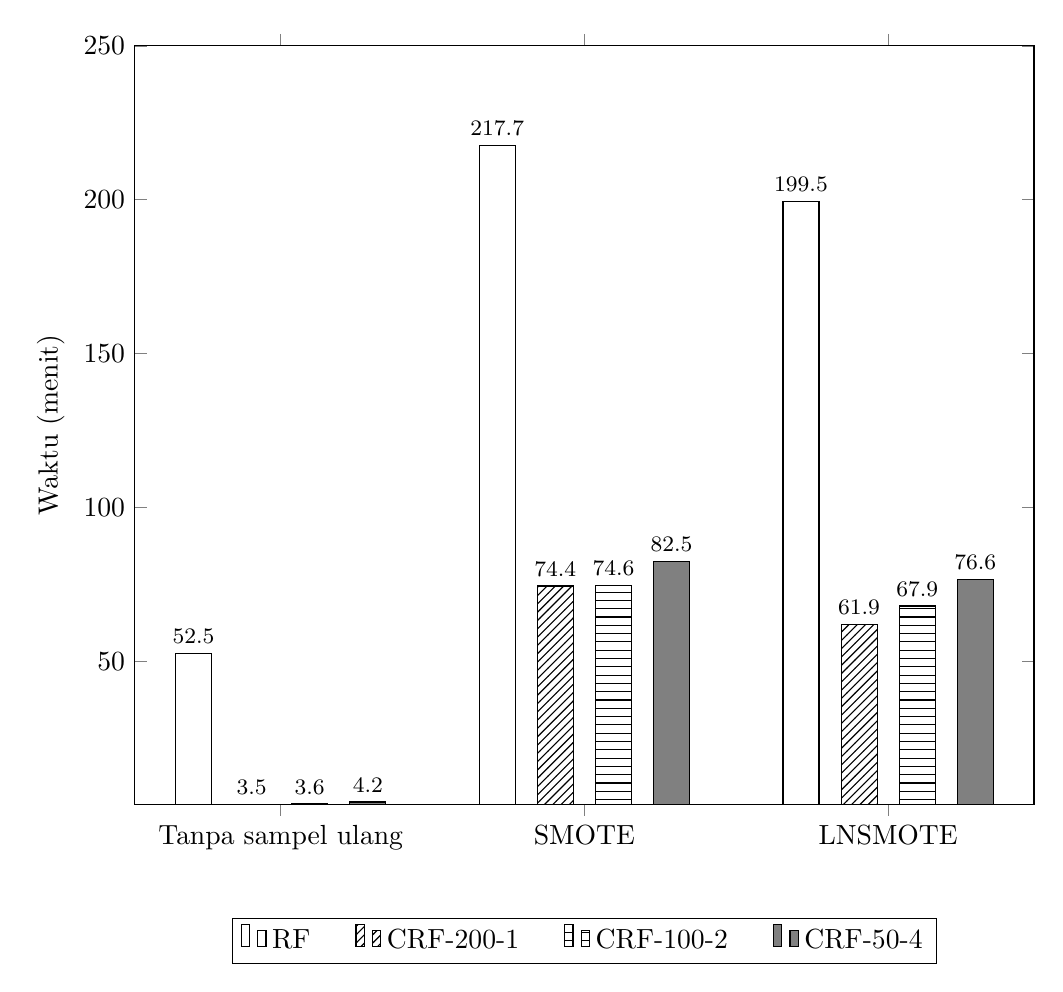
\begin{tikzpicture}
	\begin{axis}[
		width=13cm,
		ymax=250,
		ybar=8pt,
		ylabel=Waktu (menit),
		symbolic x coords={Tanpa sampel ulang, SMOTE, LNSMOTE},
		xtick=data,
		nodes near coords,
		every node near coord/.append style={font=\footnotesize},
		enlarge x limits=0.24,
		enlarge y limits=0,
		bar width = 13pt,
		legend style={
			at={(0.5,-0.15)},
			anchor=north,
			legend columns=-1,
			/tikz/every even column/.append style={column sep=0.5cm}
		},
	]
		%% RF
		\addplot[fill=white] coordinates {
			(Tanpa sampel ulang, 52.5)
			(SMOTE, 217.7)
			(LNSMOTE, 199.5)
		};

		%% CRF-200-1
		\addplot[pattern=north east lines] coordinates {
			(Tanpa sampel ulang, 3.5)
			(SMOTE, 74.4)
			(LNSMOTE, 61.9)
		};

		%% CRF-100-2
		\addplot[pattern=horizontal lines] coordinates {
			(Tanpa sampel ulang, 3.6)
			(SMOTE, 74.6)
			(LNSMOTE, 67.9)
		};

		%% CRF-50-4
		\addplot coordinates {
			(Tanpa sampel ulang, 4.2)
			(SMOTE, 82.5)
			(LNSMOTE, 76.6)
		};
	\legend{RF, CRF-200-1, CRF-100-2, CRF-50-4}
	\end{axis}
\end{tikzpicture}
\caption{Waktu pelatihan untuk setiap klasifikasi berdasarkan dataset.}
\label{graph:runtimes}
\end{figure}


Dari segi kecepatan pelatihan model, pengklasifikasi CRF lebih cepat dari RF
baik pada semua dataset pelatihan.
Sebagai pembanding, dapat dilihat pada klasifikasi RF dan CRF 50 tingkat 4
pohon.
CRF tanpa sampel ulang lebih cepat 11 kali daripada RF, dan pada sampel ulang
SMOTE dan LNSMOTE, klasifikasi CRF 1,6 kali lebih cepat daripada RF.
Kecepatan pelatihan model untuk setiap pengklasifikasi dan dataset dapat
dilihat pada gambar \ref{graph:runtimes}.


	\section{Analisis}
	\chapter{Analisis}

Hasil pelatihan dan pengujian model dianalisis dalam tiga bagian.
Pertama, analisis dari metode sampel ulang LNSMOTE, kedua, analisis terhadap
pengklasifikasi CRF, dan yang terakhir yaitu analisis terhadap hasil
keseluruhan.

\section{Analisis Sampel-ulang}

Pengaruh sampel ulang SMOTE dan LNSMOTE berbeda pada klasifikasi RF dan CRF.
Pada klasifikasi RF, sampel ulang dengan LNSMOTE lebih baik dari SMOTE dengan
meningkatnya nilai akurasi $0,4\%$.
Pada klasifikasi CRF, metode SMOTE secara keseluruhan memberikan performansi
lebih baik daripada LNSMOTE dengan nilai AUC tertinggi didapat dengan CRF 100
tingkat 2 pohon.
Perbedaan  sampel ulang dengan SMOTE dan LNSMOTE yaitu meningkatkan nilai
\textit{F-Measure} dan akurasi pada RF, sedangkan pada CRF sebaliknya, seperti
yang terlihat pada kolom \textit{F-Measure} dan akurasi di tabel
\ref{tab:stats}.
Kelemahan dari LNSMOTE yaitu meningkatkan nilai FPR dari
klasifikasi lebih tinggi dari SMOTE, seperti yang terlihat pada kurva ROC pada
gambar \ref{fig:roc} (c) dan (d).

\label{fig:roc}
\begin{figure}[htbp]
\centering
\begin{tikzpicture}
	\pgfplotsset{
		small,
	}
	\matrix{
		\begin{axis}[
			title=(a),
			ylabel=$TPR$,
			legend columns=-1,
			legend entries={Tanpa sampel ulang\ ,SMOTE\ ,LN-SMOTE},
			legend to name=roc_legend
		]
			\addplot table[
				x={FPR},
				y={TPR},
			]
			{../result/rf.csv};
			\addplot table[
				x={FPR},
				y={TPR},
			]
			{../result/rf_smote.csv};
			\addplot table[
				x={FPR},
				y={TPR},
			]
			{../result/rf_lnsmote.csv};
		\end{axis}
		&
		\begin{axis}[
			title=(b),
		]
			\addplot table[
				x={FPR},
				y={TPR},
			]
			{../result/crf_200_1.csv};
			\addplot table[
				x={FPR},
				y={TPR},
			]
			{../result/crf_200_1_smote.csv};
			\addplot table[
				x={FPR},
				y={TPR},
			]
			{../result/crf_200_1_lnsmote.csv};
			title=(b),
		\end{axis}
		\\
		\begin{axis}[
			title=(c),
			xlabel=$FPR$,
			ylabel=$TPR$,
		]
			\addplot table[
				x={FPR},
				y={TPR},
			]
			{../result/crf_100_2.csv};
			\addplot table[
				x={FPR},
				y={TPR},
			]
			{../result/crf_100_2_smote.csv};
			\addplot table[
				x={FPR},
				y={TPR},
			]
			{../result/crf_100_2_lnsmote.csv};
		\end{axis}
		&
		\begin{axis}[
			title=(d),
			xlabel=$FPR$,
		]
			\addplot table[
				x={FPR},
				y={TPR},
			]
			{../result/crf_50_4.csv};
			\addplot table[
				x={FPR},
				y={TPR},
			]
			{../result/crf_50_4_smote.csv};
			\addplot table[
				x={FPR},
				y={TPR},
			]
			{../result/crf_50_4_lnsmote.csv};
		\end{axis}
		\\
	};
\end{tikzpicture}
\ref{roc_legend}
\caption{
Kurva ROC untuk klasifikasi RF dan CRF pada tiga dataset yaitu yang
tanpa sampel ulang, yang disampel ulang dengan SMOTE dan LN-SMOTE.
(a) RF dengan 200 pohon
(b) CRF dengan 200 tingkat 1 pohon
(c) CRF dengan 100 tingkat 2 pohon
(d) CRF dengan 50 tingkat 4 pohon
}
\end{figure}


\section{Analisis CRF}

Fokus dari pengklasifikasi CRF yaitu pada pembelajaran sampel negatif.
Pada setiap tingkatan CRF, model diuji ulang dengan semua sampel negatif, yang
didapat dari proses tingkatan sebelumnya, dan hasil yang negatif dihapus dari
sampel pelatihan dan dijadikan sebagai dataset uji pada tingkatan selanjutnya.
Berbeda dengan RF, yang mana tidak ada sampel yang dihapus saat
pelatihan, CRF membuat dataset yang tadinya condong pada kelas mayoritas
sedikit demi sedikit pada setiap tingkatan menjadi sama.
Sehingga, melakukan sampel ulang pada pengklasifikasi dengan CRF tidak membantu
dalam memperbaiki performansi modelnya, namun membuat akurasi dari model hasil
pelatihan menurun.
Hal ini bisa dilihat pada kurva PR-AUC pada gambar \ref{fig:prauc}.

Pada gambar \ref{fig:prauc} (b), yaitu CRF dengan 200 tingkatan dan 1 pohon,
performansi tanpa sampel ulang lebih baik dari yang lainnya, dengan nilai AUC
$0,8673$, dan performansi yang buruk dari dataset LNSMOTE.
Saat jumlah pohon pada setiap tingkatan dinaikan menjadi 2 (dan jumlah
tingkatan diturunkan menjadi 100 supaya jumlah keseluruhan pohon tetap 200),
sampel ulang SMOTE menghasilkan nilai AUC yang paling tinggi diantara
model lainnya yaitu $0,8694$, sementara LNSMOTE masih dengan performansi yang
paling rendah, seperti yang terlihat pada gambar \ref{fig:prauc} (b).
Pada pengujian terakhir dengan 50 tingkatan dan 4 pohon, nilai AUC tertinggi
memang didapat dari SMOTE, tapi rerata performansi keseluruhan dihasilkan dari
CRF tanpa sampel ulang, dengan nilai \textit{F-Measure} yang paling tinggi
diantara pengujian lainnya yaitu $0,5353$.

\label{fig:prauc}
\begin{figure}[htbp]
\centering
\begin{tikzpicture}
	\pgfplotsset{
		small,
	}
	\matrix{
		\begin{axis}[
			title=(a),
			ylabel=$Precision$,
			legend columns=-1,
			legend entries={Tanpa sampel ulang\ ,SMOTE\ ,LN-SMOTE},
			legend to name=rf_crf_prauc_legend
		]
			\addplot table[
				x={TPR},
				y={PREC},
			]
			{../result/rf.csv};
			\addplot table[
				x={TPR},
				y={PREC},
			]
			{../result/rf_smote.csv};
			\addplot table[
				x={TPR},
				y={PREC},
			]
			{../result/rf_lnsmote.csv};
		\end{axis}
		&
		\begin{axis}[
			title=(b),
		]
			\addplot table[
				x={TPR},
				y={PREC},
			]
			{../result/crf_200_1.csv};
			\addplot table[
				x={TPR},
				y={PREC},
			]
			{../result/crf_200_1_smote.csv};
			\addplot table[
				x={TPR},
				y={PREC},
			]
			{../result/crf_200_1_lnsmote.csv};
			title=(b),
		\end{axis}
		\\
		\begin{axis}[
			title=(c),
			xlabel=$Recall$,
			ylabel=$Precision$,
		]
			\addplot table[
				x={TPR},
				y={PREC},
			]
			{../result/crf_100_2.csv};
			\addplot table[
				x={TPR},
				y={PREC},
			]
			{../result/crf_100_2_smote.csv};
			\addplot table[
				x={TPR},
				y={PREC},
			]
			{../result/crf_100_2_lnsmote.csv};
		\end{axis}
		&
		\begin{axis}[
			title=(d),
			xlabel=$Recall$,
		]
			\addplot table[
				x={TPR},
				y={PREC},
			]
			{../result/crf_50_4.csv};
			\addplot table[
				x={TPR},
				y={PREC},
			]
			{../result/crf_50_4_smote.csv};
			\addplot table[
				x={TPR},
				y={PREC},
			]
			{../result/crf_50_4_lnsmote.csv};
		\end{axis}
		\\
	};
\end{tikzpicture}
\ref{rf_crf_prauc_legend}
\caption{
Kurva PR-AUC untuk klasifikasi RF dan CRF pada tiga dataset yaitu yang
tanpa sampel ulang, yang disampel ulang dengan SMOTE dan LN-SMOTE.
(a) RF dengan 200 pohon
(b) CRF dengan 200 tingkat 1 pohon
(c) CRF dengan 100 tingkat 2 pohon
(d) CRF dengan 50 tingkat 4 pohon
}
\end{figure}


\section{Analisis Pengklasifikasi Vandalisme}

\label{fig:rocpoints}
\begin{figure}[htbp]
\centering
\begin{tikzpicture}[framed]
	\pgfplotsset{
		width=12cm,
		xtick distance=0.1,
		ytick distance=0.1,
	}
	\begin{axis}[
		title=Performansi pengklasifikasi pada ruang ROC,
		xlabel=$FPR$,
		ylabel=$TPR$,
		legend columns=3,
		legend entries={
			RF,
			RF-SMOTE,
			RF-LNSMOTE,
			CRF-200-1,
			CRF-200-1-SMOTE,
			CRF-200-1-LNSMOTE,
			CRF-100-2,
			CRF-100-2-SMOTE,
			CRF-100-2-LNSMOTE,
			CRF-50-4,
			CRF-50-4-SMOTE,
			CRF-50-4-LNSMOTE,
		},
		legend to name=class_legend
	]
		\addplot[
			scatter,
			only marks,
			point meta=explicit symbolic,
			every mark/.append style={
				/tikz/mark size=3pt
			},
			scatter/classes={
				rf-noresampling={
					mark=text,
					text mark=$\Box$
				},
				rf-smote={
					mark=text,
					text mark=$\boxplus$
				},
				rf-lnsmote={
					mark=text,
					text mark=$\boxtimes$
				},
				crf-200-1={
					mark=text,
					text mark=$\triangle$
				},
				crf-200-1-smote={
					mark=text,
					text mark=$\triangleleft$
				},
				crf-200-1-lnsmote={
					mark=text,
					text mark=$\triangleright$
				},
				crf-100-2={
					mark=text,
					text mark=$\medcircle$
				},
				crf-100-2-smote={
					mark=text,
					text mark=$\oplus$
				},
				crf-100-2-lnsmote={
					mark=text,
					text mark=$\otimes$
				},
				crf-50-4={
					mark=text,
					text mark=$\Diamond$
				},
				crf-50-4-smote={
					mark=text,
					text mark=$\diamondplus$
				},
				crf-50-4-lnsmote={
					mark=text,
					text mark=$\diamondtimes$
				}
			},
		]
		table[
			x={FPR},
			y={TPR},
			meta=klasifikasi,
		]
		{../result/cm.csv};

		\addplot[
			gray
		]
		coordinates{
			(0,0)
			(1,1)
		};
		\addplot[
			gray
		]
		coordinates{
			(0,1)
			(1,0)
		};
	\end{axis}
\end{tikzpicture}
\newline
\ref{class_legend}
\newline
\caption{
Titik ROC untuk semua pengklasifikasi dan dataset.
CRF-200-1 yaitu klasifikasi CRF
dengan 200 tingkat dan 1 pohon, CRF-100-2 yaitu klasifikasi CRF dengan 100
tingkat dan 2 pohon, dan CRF-50-4 yaitu klasifikasi CRF dengan 50 tingkat dan 4
pohon.
}
\end{figure}


Untuk lebih mudah membandingkan semua pengklasifikasi, digunakan titik
ROC yang digambarkan pada grafik \ref{fig:rocpoints}.
Pada bagian kiri bawah adalah klasifikasi RF, berurutan dari bawah ke atas
yaitu RF tanpa sampel ulang ($\Box$) dengan nilai TPR $0,165$ dan FPR $0,001$,
RF pada sampel ulang SMOTE ($\boxplus$) dengan nilai TPR $0,207$ dan FPR
$0,004$, dan yang
paling atas adalah RF pada sampel ulang LNSMOTE ($\boxtimes$) dengan nilai TPR
$0,235$ dan FPR $0,005$.
RF memberikan performansi dengan TPR dan FPR yang paling rendah di antara semua
pengklasifikasi.
Sampel ulang SMOTE meningkatkan nilai TPR $0,25$ kali dan FPR 4 kali.
Sampel ulang LNSMOTE meningkatkan nilai TPR $0,4$ kali dan nilai FPR 5 kali.

Klasifikasi CRF 200 tingkat 1 pohon (CRF-200-1) memiliki nilai TPR paling
tinggi, dengan titik ROC berada pada bagian paling atas dari semua klasifikasi.
Berurutan dari kiri ke kanan yaitu CRF-200-1 tanpa sampel ulang ($\triangle$)
dengan TPR $0,966$ dan FPR $0,467$, CRF-200-1 SMOTE ($\triangleleft$) di tengah
dengan TPR $0,979$ dan FPR $0,63$, dan CRF-200-1 LNSMOTE ($\triangleright$)
pada ujung kanan dengan TPR $0,99$ dan FPR $0,855$.
Pengklasifikasi CRF-200-1 akan mengembalikan kelas sampel positif dengan benar
tetapi dengan galat yang juga tinggi.
Bisa dilihat juga pengaruh SMOTE dan LNSMOTE terhadap nilai FPR.
Sampel ulang SMOTE memberi pengaruh kenaikan TPR $0,1$ dan $0,4$ untuk FPR dari
dataset awal.
Sampel ulang LNSMOTE meningkatkan TPR $0,3$ dan FPR $0,8$.

Klasifikasi CRF 100 tingkat dengan 2 pohon (CRF-100-2) berada pada bagian atas
tengah dari ROC, yang ditandai dengan marka bulat.
CRF-100-2 tanpa sampel ulang ($\medcircle$) berada paling bawah dan kiri dengan
nilai TPR $0,812$ dan FPR $0,24$.
CRF-100-2 SMOTE ($\oplus$) berada di tengah dengan nilai AUC paling tinggi
dengan TPR $0,903$ dan FRP $0,3603$.
CRF-100-2 LNSMOTE ($\otimes$) dengan TPR paling tinggi dari keduanya yaitu TPR
$0,953$ dan FPR $0,585$.
Sampel ulang SMOTE meningkatkan TPR $0,11$ kali dan FPR $0,5$ kali.
Sampel ulang LNSMOTE meningkatkan TPR $0,17$ dan FPR $1,4$ kali.

Klasifikasi CRF 50 tingkat dengan 4 pohon (CRF-50-4) berada pada bagian tengah
kiri atas pada ROC, yang ditandai dengan marka wajik.
CRF-50-4 tanpa sampel ulang ($\Diamond$) menghasilkan nilai TPR $0,607$ dan FPR
$0,08$.
CRF-50-4 dengan sampel ulang ($\diamondplus$) SMOTE meningkatkan nilai TPR
menjadi $0,783$ dan meningkatkan nilai FPR menjadi $0,223$.
CRF-50-4 dengan sampel ulang LNSMOTE ($\diamondtimes$) meningkatan nilai TPR
menjadi $0,895$ dan juga meningkatkan nilai FPR menjadi $0,388$.
Sampel ulang dengan SMOTE meningkatkan nilai TPR $0,3$ kali dan FPR $1,75$
kali.
Sampel ulang dengan LNSMOTE meningkatkan nilai TPR $0,48$ kali dan FPR $3,75$.



%%
%% BAB V: KESIMPULAN
%%
\chapter{Kesimpulan}

Secara keseluruhan, performansi dari sampel ulang LNSMOTE lebih baik daripada
SMOTE untuk kedua pengklasifikasi.
Pengaruh menarik lainnya yaitu pada pengklasifikasi CRF, dengan menggunakan
jumlah pohon lebih sedikit pada setiap tingkatan menghasilkan performansi yang
hampir sama dengan melakukan sampel ulang pada dataset asli, seperti yang
terlihat pada performansi CRF 100 tingkat 2 pohon pada dataset tanpa sampel
ulang, hampir sama dengan CRF 50 tingkat 4 pohon dengan sampel ulang SMOTE.

Untuk model klasifikasi vandalisme yang terbaik tanpa sampel ulang dihasilkan
dari pengklasifikasi CRF dengan 200 tingkat dan 1 pohon dengan nilai TPR
$0,9668$,
untuk model terbaik pada dataset yang telah disampel ulang dengan SMOTE yaitu
CRF dengan 200 tingkat dan 1 pohon dengan nilai TPR $0,9790$,
dan untuk model terbaik dari sampel ulang LNSMOTE yaitu CRF dengan 200 tingkat
1 pohon dengan nilai TPR $0.9904$.
Secara keseluruhan model terbaik yaitu dari CRF 200 tingkat dan 1 pohon yang
telah disampel ulang dengan LNSMOTE.
Selain performansi yang lebih baik, pengklasifikasi CRF juga lebih cepat $1,6$
kali dalam pembentukan model daripada RF pada dataset yang telah disampel
ulang.

\section{Kontribusi}

Kontribusi dari karya tulis ini selain membantu menemukan pengklasifikasi yang
lebih baik dalam mendeteksi vandalisme juga memberikan kerangka kerja untuk
menciptakan dan mengembangkan fitur vandalisme dari dataset mentah tanpa harus
mulai dari awal untuk dapat digunakan dalam penelitian selanjutnya atau
digunakan langsung pada kasus asli. Selain itu juga menyediakan pustaka program
untuk pengolahan data dan fungsi pembelajaran mesin terutama untuk sampel ulang
LNSMOTE dan pengklasifikasi
\textit{Cascaded Random Forest} yang belum ada implementasi secara terbuka pada
program terkenal seperti \textit{Weka}, \textit{Scikit-Learn}, atau \textit{R}.

\section{Pekerjaan Selanjutnya}

Jumlah artikel Bahasa Indonesia di Wikipedia setiap tahun semakin meningkat
seiring dengan bertambahnya jumlah pengguna internet di Indonesia.
Semakin banyak pengguna, kemungkinan vandalisme juga semakin tinggi.
Untuk mengatasi masalah vandalisme tersebut lebih awal, akan lebih baik bila
disiapkan sebuah sistem untuk mendeteksi vandalisme pada Wikipedia
Bahasa Indonesia.
Langkah awalnya bisa dengan mengumpulkan data artikel yang telah dianotasi
dengan vandal, supaya dapat dianalisis untuk pembuatan fitur dan pembuatan
model deteksi vandalisme pada Wikipedia Bahasa Indonesia.

Semua pelatihan model dalam karya tulis ini masih menggunakan algoritma
pengklasifikasi RF dan CRF dalam bentuk serial, yang mana satu pohon dibangun
satu per satu bergantian atau pada saat klasifikasi setiap sampel dimasukan ke
dalam pohon secara bergantian untuk mendapatkan kelasnya.
Penggunaan algoritma paralel, seperti dalam pembentukan dua atau empat pohon
bersamaan dan klasifikasi sampel (pengumpulan kelas di setiap pohon)
bersamaan, bisa membantu mempercepat pelatihan, pengujian dan hasil
klasifikasi.
Pada domain pembelajaran mesin, hal menarik yaitu adanya algoritma
\textit{eXtreme Gradient Boostring} (XGBoost)
\parencite{chen2016xgboost}
yang
mungkin bisa meningkatkan deteksi vandalisme.


%%
%% DAFTAR PUSTAKA
%%
\chapter*{\vspace{0em}\tDaftarPustaka}
	\addcontentsline{toc}{chapter}{\tDaftarPustaka}
	\printbibliography

%%
%% LAMPIRAN
%%
\clearpage
\vspace*{\fill}
\begin{center}
	\begin{minipage}{\textwidth}
		\chapter*{\vspace{0em}\tUpLampiran}
		\addcontentsline{toc}{chapter}{\tUpLampiran}
	\end{minipage}
\end{center}
\vfill

\vspace*{\fill}
\begin{center}
	\begin{minipage}{\textwidth}
		\centering
		\textbf{\Large\tUpLampiran}
		\addcontentsline{toc}{chapter}{\tUpLampiran}
	\end{minipage}
\end{center}
\vfill

\myappendix{Daftar Kategori Kata dan Token}
	\label{lampiran:daftar_token_dan_kata}

\subappendix{Sintaks Wiki}
\label{lampiran:words_wiki_token}

Kategori sintaks wiki digunakan dalam penghitungan fitur \textit{token umum}.
Berikut daftar token yang digunakan,

\begin{lstlisting}
"=", "==", "===", "====", "=====",
":", "::", ":::", "::::", ":::::", "::::::",
"*", "**", "***", "****",
"#", "##", "###", "####",
";",
"''", "'''", "'''''",
"----",
"__FORCETOC__", "__TOC___", "__NOTOC__",
"<blockquote", "blockquote>",
"<div", "/div>",
"<code", "/code>",
"<syntaxhighlight", "/syntaxhighlight>",
"<small", "/small>",
"<big", "/big>",
"<pre", "/pre>",
"<nowiki", "/nowiki>",
"<sub", "/sub>",
"<sup", "/sup>",
"<math", "/math>",
"<ref", "/ref>",
"{{", "}}",
"[[", "]]",
"{{cite book", "{{cite web",
"{{Help:",
"~~~", "~~~~", "~~~~~",
"[[Special:", "[[media:", "[[Media:", "[[File:",
"[[Wikipedia", "[[Wiktionary:", "[[Category:",
"[http://",
"ISBN ", "#REDIRECT"
\end{lstlisting}

\subappendix{Kategori Kata Vulgar}
\label{lampiran:words_vulgar}

Kategori kata vulgar yaitu kata yang kasar dan menghina.
Berikut daftar kata vulgar yang digunakan,

\begin{lstlisting}
"$#!+", "$1ut", "$h1t", "$hit", "$lut", "'f*ck'", "'ho", "'hobag",
"@ss", "@sshole", "a$$", "a$$h0!e", "a$$h01e", "a$$h0le", "a$$hole",
"a55", "a55hole", "aeolus", "ahole", "analprobe", "anilingus",
"anorexia", "anorexic", "anus", "areola", "areole", "arian", "aryan",
"ass", "assbang", "assbanged", "assbangs", "asses", "assfuck",
"assfucker", "assfuckers", "assh0le", "assho!e", "assho1e", "asshole",
"assholes", "assmaster", "assmunch", "asswipe", "asswipes", "azazel",
"azz", "b1tch", "b1tch", "b@lls", "baal", "babe", "babes", "ballsack",
"bang", "banger", "barf", "bastard", "bastards", "bawdy", "beaner",
"beardedclam", "beastiality", "beatch", "beater", "beaver", "beer",
"beeyotch", "beotch", "biatch", "bigtits", "bimbo", "bitch", "bitched",
"bitches", "bitchface", "bitchy", "blew", "blow", "blow", "blowjob",
"blowjobs", "blowup", "bod", "bodily", "boink", "bollock", "bollocks",
"bollok", "bone", "boned", "boner", "boners", "bong", "boob",
"boobies", "boobs", "booby", "booger", "bookie", "booky", "bootee",
"bootie", "booty", "booze", "boozer", "boozy", "bosom", "bosomy",
"bowel", "bowels", "bra", "brassiere", "bugger", "bukkake", "bulimia",
"bulimiic", "bullshit", "bullshits", "bullshitted", "bullturds",
"bung", "burp", "bush", "busty", "butt", "buttfuck", "buttfucker",
"buttplug", "c-0-c-k", "c-o-c-k", "c-u-n-t", "c.0.c.k", "c.o.c.k.",
"c.u.n.", "c0ck", "caca", "cahone", "cameltoe", "carnal",
"carpetmuncher", "cawk", "cervix", "chinc", "chincs", "chink", "chink",
"chode", "chodes", "cl1t", "climax", "clit", "clit", "clitoris",
"clitorus", "clits", "clitty", "cocain", "cocaine", "cock",
"cockblock", "cockholster", "cockknocker", "cocks", "cocksucker",
"coital", "coke", "commie", "condom", "coon", "coons", "copulator",
"corksucker", "corpse", "coven", "crabs", "crack", "cracker",
"crackwhore", "crap", "crappy", "cuervo", "cum", "cummin", "cumming",
"cumshot", "cumshots", "cumstain", "cunilingus", "cunnilingus",
"cunny", "cunt", "cuntface", "cunthunter", "cuntlick", "cuntlicker",
"cunts", "d0ng", "d0uch3", "d0uche", "d1ck", "d1ck", "d1ld0", "d1ldo",
"dago", "dagos", "dammit", "damn", "damned", "damnit", "dawgie-style",
"dick", "dick-ish", "dickbag", "dickdipper", "dickflipper", "dickhead",
"dickheads", "dickish", "dickripper", "dicksipper", "dickweed",
"dickwhipper", "dickzipper", "diddle", "dike", "diligaf", "dillweed",
"dimwit", "dingle", "doggie", "doggie-style", "doggy", "doggy-style",
"dong", "doofus", "doosh", "dopey", "douch3", "douche", "douche",
"douchebag", "douchebags", "douchey", "drunk", "dumass", "dumbass",
"dumbasses", "dummy", "dyke", "dykes", "ejaculate", "enlargement",
"erect", "erotic", "essohbee", "exotic", "extacy", "extasy", "f-u-c-k",
"f.u.c.k", "f@g", "f@gg0t", "f@ggot", "fack", "faerie", "faery", "fag",
"fagg", "fagged", "faggit", "faggot", "fagot", "fags", "faig", "faigt",
"fairy", "fanny", "fannybandit", "fart", "fartknocker", "felch",
"felcher", "felching", "fellate", "fellatio", "fellatio", "feltch",
"feltcher", "fisted", "fisting", "fisty", "floozy", "foad", "fondle",
"foobar", "foreskin", "frack", "freex", "frigg", "frigga", "fu*ck",
"fubar", "fuck", "fuck-tard", "fucka$$", "fuckass", "fucked", "fucker",
"fucker", "fuckers", "fuckface", "fucking", "fucknugget", "fucknut",
"fuckoff", "fucks", "fucktard", "fuckup", "fuckwad", "fuckwit",
"fudgepacker", "fuk", "futs", "fvck", "fxck", "g-spot", "g@y", "gae",
"gai", "ganja", "gay", "gays", "gey", "gfy", "ghay", "ghey", "gigolo",
"glans", "goatse", "godamn", "godamnit", "godamnit", "goddam",
"goddammit", "goddamn", "goldenshower", "gonad", "gonads", "gonads",
"gook", "gooks", "gspot", "gtfo", "h0m0", "h0mo", "handjob", "he11",
"hebe", "hell", "hemp", "heroin", "herp", "herpes", "herpy", "hijack",
"hitler", "hiv", "hobag", "hom0", "homey", "homo", "homoey", "honky",
"hooch", "hookah", "hooker", "hoor", "hootch", "hooter", "hooters",
"horny", "hump", "humped", "humper", "humping", "hussy", "hymen",
"idiot", "idiots", "inbred", "incest", "injun", "j3rk0ff", "jackass",
"jackhole", "jackoff", "jap", "japs", "jerk", "jerk", "jerk0ff",
"jerked", "jerkoff", "jism", "jiz", "jizm", "jizm", "jizz", "jizzed",
"junkie", "junky", "kike", "kikes", "kill", "kinky", "kkk", "klan",
"knobend", "knobend", "kooch", "kooches", "kootch", "kraut", "kyke",
"labia", "lech", "leper", "lesbians", "lesbos", "lez", "lezbian",
"lezbians", "lezbo", "lezbos", "lezzie", "lezzies", "lezzy", "licker",
"lickers", "lmao", "lmfao", "loin", "loins", "lsd", "lube", "lust",
"lusty", "m-fucking", "mams", "marijuana", "massa", "masterbate",
"masterbating", "masterbation", "masturbate", "masturbating",
"masturbation", "maxi", "menses", "menstruate", "menstruation", "meth",
"mofo", "molest", "moolie", "moron", "motherf*cker", "motherfucka",
"motherfucker", "motherfucking", "mtherfucker", "mthrf*cker",
"mthrfucker", "mthrfucking", "muff", "murder", "muthafuckaz",
"muthafucker", "mutherfucker", "mutherfucking", "muthrfucking", "nad",
"nads", "naked", "napalm", "nappy", "nazi", "nazism", "negro", "nigga",
"niggah", "niggas", "niggaz", "nigger", "niggers", "niggle", "nimrod",
"ninny", "nooky", "nucking", "nympho", "opiate", "opium", "oral",
"orally", "organ", "orgasm", "orgasmic", "orgies", "orgy", "ovary",
"ovum", "ovums", "p*ssy", "p.u.s.s.y.", "p.u.s.s.y.", "paddy",
"paedophile", "pantie", "panties", "panty", "pastie", "pasty", "pcp",
"pecker", "pedo", "pedophile", "pedophile", "pedophiles", "pedophilia",
"pedophiliac", "pee", "peepee", "penetrate", "penetration", "penial",
"penile", "perversion", "peyote", "phalli", "phallic", "phuck",
"pillowbiter", "pimp", "pinko", "piss", "piss-off", "pissed",
"pissoff", "pms", "polack", "porn", "porno", "pornography", "pot",
"potty", "prick", "prig", "prostitute", "prude", "pu$$y", "pube",
"pubic", "pubis", "punkass", "punky", "puss", "pussies", "pussy",
"pussypounder", "pussys", "queaf", "queef", "queefing", "queer",
"queero", "queers", "quicky", "quife", "quim", "r-tard", "racist",
"racy", "rape", "raped", "raper", "rapist", "raunch", "rectal",
"rectum", "rectus", "reefer", "reetard", "reich", "retard", "retarded",
"revue", "rim", "risque", "ritard", "rtard", "rum", "rump",
"rumprammer", "s***", "s*o*b", "s-h-1-t", "s-h-i-t", "s-o-b",
"s.h.i.t.", "s.o.b.", "s0b", "sadism", "sadist", "satan", "scag",
"scantily", "schizo", "screw", "screwed", "scrog", "scrot", "scrote",
"scrotum", "scrud", "scum", "seaman", "seamen", "seduce", "semen",
"sex_story", "sexual", "sh!t", "sh*t", "sh1t", "shamedame", "shit",
"shite", "shiteater", "shitface", "shithead", "shithole", "shithouse",
"shits", "shitt", "shitted", "shitter", "shitty", "shiz", "sissy",
"skag", "slave", "sleaze", "sleazy", "slut", "slutdumper", "slutkiss",
"sluts", "smegma", "smut", "smutty", "snatch", "sniper", "snuff",
"sodom", "souse", "soused", "sperm", "spic", "spick", "spik", "spiks",
"spooge", "spunk", "stab", "steamy", "stfu", "stiffy", "stoned",
"strip", "stroke", "suck", "sucked", "sucking", "sucks",
"sumofabiatch", "t1t", "tampon", "tard", "tawdry", "teabagging",
"teat", "terd", "teste", "testee", "testes", "testis", "thrust",
"thug", "tinkle", "tit", "titfuck", "titi", "tits", "tittiefucker",
"titties", "titty", "tittyfuck", "tittyfucker", "toke", "toots",
"tosser", "tossers", "tramp", "transsexual", "trashy", "tubgirl",
"turd", "tush", "twat", "twats", "undies", "unwed", "urinal", "urine",
"uterus", "uzi", "vag", "valium", "viagra", "virgin", "vixen", "vodka",
"vomit", "voyeur", "vulgar", "vulva", "w@ng", "wad", "wang", "wank",
"wazoo", "wedgie", "weed", "weenie", "weewee", "weiner", "weirdo",
"wench", "wetback", "wh0r3f@ce", "wh0re", "wh0ref@ce", "wh0reface",
"whack", "whacked", "whacking", "whitey", "whiz", "whoralicious",
"whore", "whorealicious", "whored", "whoreface", "whorehopper",
"whorehouse", "whores", "whoring", "wigger", "womb", "woody", "wop",
"wtf", "x-rated", "xxx", "yeasty", "yobbo", "zoophile"
\end{lstlisting}

\subappendix{Kategori Kata Subjek}
\label{lampiran:words_pronoun}

Kategori kata subjek yaitu kata yang merujuk pada pihak pertama dan kedua yang
digunakan dalam percakapan sehari-hari.
Berikut daftar kata subjek yang digunakan,

\begin{lstlisting}
"i", "me", "mine", "my", "myself", "our", "ours", "ourself",
"ourselves", "selves", "thee", "thine", "thou", "thy", "thyself", "us",
"we", "y'all", "y'all", "y'all's", "yis", "you", "you-uns", "your",
"yours", "yourself", "yourselves", "yourselves", "yous", "yous's",
"youse", "youse"
\end{lstlisting}


\subappendix{Kategori Kata Bias}
\label{lampiran:words_bias}

Kategori kata bias berisi kata yang mengesankan penekanan yang berlebihan
sehingga cenderung membuat bias.
Berikut daftar kata bias yang digunakan,

\begin{lstlisting}
"cutting-edge", "single-handedly", "well-established", "well-known",
"world-class", "absolute", "acclaimed", "amazing", "astonishing",
"authoritative", "beautiful", "best", "boreing", "boring", "brilliant",
"canonical", "cares", "celebrated", "charismatic", "classic",
"coolest", "defining", "definitive", "eminent", "enigma", "ever",
"everyone", "exciting", "extraordinary", "fabulous", "famous",
"fantastic", "fat", "fully", "genius", "global", "great", "greatest",
"hate", "huge", "iconic", "idiotic", "immensely", "impactful",
"incendiary", "indisputable", "infamous", "influential", "innovative",
"inspired", "intriguing", "lame", "leader", "leading", "legendary",
"like", "major", "masterly", "mature", "memorable", "most", "notable",
"outstanding", "pioneer", "popular", "prestigious", "probably",
"really", "remarkable", "renowned", "respected", "seminal",
"significant", "skillful", "solution", "staunch", "strange", "super",
"talented", "top", "total", "totally", "transcendent", "ugly",
"undoubtedly", "unique", "virtually", "virtuoso", "visionary", "weird",
"worst"
\end{lstlisting}

\subappendix{Kategori Kata Pornografi}
\label{lampiran:words_sex}

Berikut daftar kata pornografi yang digunakan,

\begin{lstlisting}
"anal", "breast", "breasts", "buttocks", "dildo", "dildos", "erect",
"nipple", "nipples", "penis", "sex", "sodomized", "sodomy", "vagina",
"vibrator", "vibrators"
\end{lstlisting}

\subappendix{Kategori Kata Buruk}
\label{lampiran:words_bad}

Kategori kata buruk mengikutkan kata-kata yang bersifat negatif, bukan vulgar
dan bukan pornografi, atau kata slang yang digunakan dalam sehari-hari.
Berikut daftar kata buruk yang digunakan,

\begin{lstlisting}
"666", "da", "dont", "dosent", "whatever", "guy", "hi", "nazi", "sup",
"guise", "loser", "thats", "ugly", "wanna", "whats", "wont", "gotta",
"bloody", "fart", "pot", "prick", "stink", "smells", "smelly", "alot",
"dunno", "gotcha"
\end{lstlisting}



\myappendix{Contoh Dataset}
	\label{lampiran:dataset}

\subappendix{Dataset Suntingan PAN-WVC-10}
	\label{lampiran:dataset_wvc10_suntingan}

Berikut contoh dataset suntingan pada PAN-WVC-10,

\lstinputlisting[style=data,basicstyle=\footnotesize\ttfamily]
	{lampiran/dataset_wvc10_suntingan}

\subappendix{Dataset Anotasi PAN-WVC-10}
	\label{lampiran:dataset_wvc10_anotasi}

Berikut contoh dataset anotasi pada PAN-WVC-10,

\lstinputlisting[style=data,basicstyle=\footnotesize\ttfamily]
	{lampiran/dataset_wvc10_anotasi}

\subappendix{Dataset Gabungan PAN-WVC-10}
	\label{lampiran:dataset_wvc10_gabungan}

Berikut contoh dataset PAN-WVC-10 yang telah dibersihkan dan ditambahkan dengan
atribut \textit{additions} dan \textit{deletions},

\lstinputlisting[
	style=data
,	basicstyle=\footnotesize\ttfamily
,	texcl=true
]{lampiran/dataset_wvc10_gabungan}

\subappendix{Dataset Mentah PAN-WVC-11}
	\label{lampiran:dataset_wvc11_mentah}

Berikut contoh dataset mentah dari PAN-WVC-11 Bahasa Inggris,

\lstinputlisting[
	style=data
,	basicstyle=\footnotesize\ttfamily
,	texcl=true
]{lampiran/dataset_wvc11_mentah}

\subappendix{Dataset Gabungan PAN-WVC-11}
	\label{lampiran:dataset_wvc11_gabungan}

Berikut contoh dataset PAN-WVC-11 yang telah dibersihkan dan ditambahkan
atribut \textit{additions} dan \textit{deletions},

\lstinputlisting[
	style=data
,	basicstyle=\footnotesize\ttfamily
,	texcl=true
,	alsoletter={\\}
,	morekeywords={\"}
]{lampiran/dataset_wvc11_gabungan}


\end{document}
